\documentclass[12pt,english,brazil,a4paper,utf8,oneside]{utfpr-tcc}
\usepackage{float}

% carrega o arquivo configuracoes.tex que contém os pacotes e comandos Latex.
%
% Esse arquivo conterá pacotes e comandos utilizados na monografia
%
% Observação - devido a um erro do sharelatex foi necessário colocar na raiz do projeto os seguintes arquivos:
% gcnumparser.sty, fcprefix.sty, fmtcount.sty, fc-poruges.def, fcportuguese.def.
% Tal problema foi relatado em: https://github.com/nlct/fmtcount/issues/26
% Quando o sharelatex corrigir o problema acredito que podemos remover esses arquivos do projeto. At. Luiz Arthur.
%

% Este comando não é necessário: utilizei apenas para deixar o latex2rtf
% feliz (e descobrir a codificação do texto).
\usepackage[utf8]{inputenc}

% Suporte a figuras e subfiguras
\usepackage{graphics}
\usepackage{subfigure}

% Suporte a tabelas (principalmente do cronograma)
\usepackage{tabularx}
\usepackage{multirow}
\usepackage{array}
\usepackage{tabularx}
\usepackage{colortbl}
\usepackage{hhline}
\usepackage{xcolor}

% Escalar fontes para redimencionar, por exemplo tabelas
\usepackage{scalefnt}

% Algoritmos.
\usepackage{algorithm,algorithmic}

\usepackage[alf]{abntex2cite}

% Elementos geralmente utilizados na tabela do cronograma
\newcommand{\fullcell}{\multicolumn{1}{>{\columncolor[gray]{0.5}}c}{}}
\newcommand{\fullcellline}{\multicolumn{1}{>{\columncolor[gray]{0.5}}c|}{}}
\newcommand{\mc}[3]{\multicolumn{#1}{#2}{#3}}
\newcommand{\y}{\rule{8pt}{4pt}}
\newcommand{\n}{\hspace*{8pt}}

% Define o caminho das figuras
\graphicspath{{images/}}

%% Configuração de glossário
\usepackage[portuguese]{nomencl}
\usepackage[nogroupskip,acronym,nomain,nonumberlist,nopostdot,nohypertypes={acronym}]{glossaries}

\makenoidxglossaries

% para siglas em português
\newcommand{\sigla}[2]
{
 \newglossaryentry{#1}{
  name=#1,
  description={#2},
  first={#2 (#1)},
  long={#2}
 }  
}

% para siglas de língua estrangeira, nessas a descrição longa fica em itálico.
\newcommand{\siglaIt}[2]
{
 \newglossaryentry{#1}{
  name=#1,
  description={\textit{#2}},
  first={\textit{#2} ({#1})},
  long={\textit{#2}}
 }  
}

% --- Estilos para apresentação de Código ----- %
\usepackage{listings}
\lstloadaspects{formats}

% Opções de listing usados para o código fonte
% Ref: http://en.wikibooks.org/wiki/LaTeX/Packages/Listings

\lstset{ %
language=Java,                  % choose the language of the code
basicstyle=\footnotesize,       % the size of the fonts that are used for the code
%basicstyle=\ttfamily,
stringstyle=\ttfamily\color[rgb]{0.16,0.16,0.16},
numbers=left,                   % where to put the line-numbers
numberstyle=\footnotesize,      % the size of the fonts that are used for the line-numbers
stepnumber=1,                   % the step between two line-numbers. If it's 1 each line will be numbered
numbersep=4pt,                  % how far the line-numbers are from the code
showspaces=false,               % show spaces adding particular underscores
showstringspaces=false,         % underline spaces within strings
showtabs=false,                 % show tabs within strings adding particular underscores
frame=single,	                % adds a frame around the code
framerule=0.6pt,
tabsize=2,	                % sets default tabsize to 2 spaces
captionpos=b,                   % sets the caption-position to bottom
breaklines=true,                % sets automatic line breaking
breakatwhitespace=false,        % sets if automatic breaks should only happen at whitespace
escapeinside={\%*}{*)},         % if you want to add a comment within your code
backgroundcolor=\color[rgb]{1.0,1.0,1.0}, % choose the background color.
rulecolor=\color[rgb]{0.8,0.8,0.8},
extendedchars=true,
xleftmargin=10pt,
xrightmargin=10pt,
framexleftmargin=10pt,
framexrightmargin=10pt
}

\definecolor{javared}{rgb}{0.6,0,0} % for strings
\definecolor{javagreen}{rgb}{0.25,0.5,0.35} % comments
\definecolor{javapurple}{rgb}{0.5,0,0.35} % keywords
\definecolor{javadocblue}{rgb}{0.25,0.35,0.75} % javadoc

\definecolor{DarkBlue}{rgb}{0,0,0.61}
\definecolor{DarkGreen}{rgb}{0,0.4,0}

% Numeros.
\lstdefinestyle{mynumbers}{
	numbers=left,
	stepnumber=1,
	numbersep=4pt,
	numberstyle=\tiny\color{black}
}
% Text Code.
\lstdefinestyle{mytextcode}{
	basicstyle=\footnotesize,
	tabsize=2,
	showspaces=false,
	showstringspaces=false,
	extendedchars=true,
	breaklines=true
}
% Frame.
\lstdefinestyle{myframe}{
	backgroundcolor=\color{white},
	frame=trbl
}
% C++ Style.
\lstdefinestyle{C++}{
	language=C++,
	style=mynumbers,
	style=mytextcode,
	style=myframe,
  keywordstyle=\color{black}\bfseries,
  stringstyle=\color{gray},
  commentstyle=\color[rgb]{0.08,0.08,0.08},
  morecomment=[s][\color{lightgray}]{/*}{*/},
  otherkeywords={\#include, \#define, \#pragma, \#typedef, dim3},
  emph={ __device__, __global__, __shared__, __host__, __constant__},
  emphstyle=\color{DarkBlue}\bfseries,
  emph={[2] printf, scanf},
  emphstyle=[2]\color{DarkGreen},
}
% C Style.
\lstdefinestyle{C}{
	language=C,
	style=mynumbers,
	style=mytextcode,
	style=myframe,
	keywordstyle=\color{black}\bfseries,
  	stringstyle=\color{gray},
  	commentstyle=\color[rgb]{0.08,0.08,0.08},
  	morecomment=[s][\color{lightgray}]{/*}{*/},
  	otherkeywords={\#include, \#define, \#pragma, \#typedef, dim3, bool},
  	emph={ __device__, __global__, __shared__, __host__, __constant__},
  	emphstyle=\color{DarkBlue}\bfseries,
  	emph={[2] printf, scanf},
  	emphstyle=[2]\color{DarkGreen},
	backgroundcolor={}
}
% Bash Style.
\lstdefinestyle{bash}{
	language=bash,
	style=mynumbers,
	style=mytextcode,
	style=myframe,
	backgroundcolor={},
	frame=single,
	basicstyle=\scriptsize\ttfamily
}
% Python Style.
\lstdefinestyle{python}{
	language=python,
	style=mynumbers,
	style=mytextcode,
	style=myframe,
	backgroundcolor={}
}
% Java Style.
\lstdefinestyle{java}{
	language=java,
	style=mynumbers,
	style=mytextcode,
	style=myframe,
	backgroundcolor={}
}
% ASM Style.
\lstdefinestyle{asm}{
  %belowcaptionskip=1\baselineskip,
  %xleftmargin=\parindent,
  language=[x86masm]Assembler,
  style=mynumbers,
  style=mytextcode,
  style=myframe,
  backgroundcolor={},
  frame=single,
  basicstyle=\scriptsize\ttfamily,
  commentstyle=\itshape\color{purple!40!black},
}

% Fortran Style.
\lstdefinestyle{fortran}{
  language=[90]Fortran,
  style=mynumbers,
  style=mytextcode,
  style=myframe,
  backgroundcolor={},
  frame=single,
  basicstyle=\footnotesize,
  commentstyle=\itshape\color{purple!40!black},
  morecomment=[l]{!\ }% Comment only with space after !
}

% LLVM Style.
\lstdefinestyle{llvm}{
	language=llvm,
	%inputencoding=utf8,
	style=mynumbers,
	style=mytextcode,
	style=myframe,
	backgroundcolor={},
	frame=single,
	basicstyle=\scriptsize\ttfamily,
  tabsize=4,
  %rulecolor=,
  upquote=true,
% aboveskip={1.5\baselineskip},
  columns=fixed,
  prebreak = \raisebox{0ex}[0ex][0ex]{\ensuremath{\hookleftarrow}},
  showtabs=false,
	%basicstyle=\scriptsize\upshape\ttfamily,
  identifierstyle=\ttfamily,
  keywordstyle=\ttfamily\bfseries\color[rgb]{0,0,0},
  %commentstyle=\ttfamily\color[rgb]{0.133,0.545,0.133},
  commentstyle=\ttfamily\color[rgb]{0.08,0.08,0.08},
  %stringstyle=\ttfamily\color[rgb]{0.627,0.126,0.941}
  stringstyle=\ttfamily\color[rgb]{0.16,0.16,0.16}
}

\lstdefineformat{C}{%
	\{=\newline\string\newline\indent,%
	\}=[;]\newline\noindent\string\newline,%
	\};=\newline\noindent\string\newline,%
	;=[\ ]\string\space}

% --- Fim da Definição de Estilos para apresentação de Código ----- %
% carrega o arquivo constantes.tex que contém dados do curso/monografia que NÃO DEVEM ser alterados. 
% Dados do curso que não precisam de alteração
\university{Universidade Tecnológica Federal do Paraná}
\universityen{Federal University of Technology -- Paraná}
\universityunit{Departamento Acadêmico de Computação}
\address{Campo Mourão}
\addressen{Campo Mourão, PR, Brazil}
\documenttype{Monografia}
\documenttypeen{Monograph}
\degreetype{Graduação}
% carrega o arquivo variaveis.tex que contém dados do acadêmico/monografia que DEVEM ser alterados.
% Dados do curso. Caso seja BCC:
\program{Curso de Bacharelado em Ciência da Computação}
\programen{Undergradute Program in Computer Science}
\degree{Bacharel}
\degreearea{Ciência da Computação}
% Caso seja TSI:
% \program{Curso Superior de Tecnologia em Sistemas para Internet}
% \programen{Undergradute Program in Tecnology for Internet Systems}
% \degree{Tecnólogo}
% \degreearea{Tecnologia em Sistemas para Internet}


% Dados da disciplina. Escolha uma das opções e a descomente:
% TCC1:
\goal{Proposta de Trabalho de Conclusão de Curso de Graduação}
\course{Trabalho de Conclusão de Curso 1}
% TCC2:
% \goal{Trabalho de Conclusão de Curso de graduação}
% \course{Trabalho de Conclusão de Curso 2}


% Dados do TCC (precisa alterar)
\author{Clodoaldo Adão Basaglia da Fonseca}  % Seu nome
\title{Veículo autônomo terrestre de baixo custo para uso agrícola} % Título do trabalho
\titleen{} % Título traduzido para inglês
\advisor{Prof. Dr. Radames Juliano Halmeman } % Nome do orientador. Lembre-se de prefixar com "Prof. Dr.", "Profª. Drª.", "Prof. Me." ou "Profª. Me."}
% \coadvisor{} % Nome do coorientador, caso exista. Caso não exista, comente a linha.
\depositshortdate{2018} % Ano em que depositou este documento

% Dados da ficha catalografica. Ela é opcional, mas é uma boa ideia inserí-la. Exemplos para geração (http://fichacatalografica.sibi.ufrj.br/)
\fichacatautor{}  % Nome conforme citado (ou seja, no formato "Sobrenome, Nome").
\fichacatbib{Biblioteca da UTFPR de Campo Mourão} % Não alterar
\fichacatpum{M488} % Código Cutter-Sanborn. Use a primeira letra do sobrenome seguido do número conforme as primeiras letras do sobrenome e a tabela http://www.amormino.com.br/cutter-sanborn/cutter1.html
\fichacatpalcha{} % Assuntos do trabalho. Cada item deve ser enumerado e separado por ponto: 1. xxx. 2. yyy. 3. zzz.
\fichacatpdois{} % Deixar em branco

% carrega o arquivo listaabreviaturas.tex que está dentro do diretório pretextual, esse arquivo contém as siglas utilizadas na monografia.
% quando a sigla for de língua portuguesa utilize \sigla{SIGLA}{Significado em português}
% quando a sigla for de língua estrangeira utilize \siglaIt{SIGLA}{Significado em Inglês}

\sigla{UTFPR}{Universidade Tecnológica Federal do Paraná}
\siglaIt{ACM}{Association for Computing Machinery}
\siglaIt{IP}{Internet Protocol}


% No texto quando for utilizar a sigla utilize os seguintes comandos:
%\acrlong{label} - acronimo/sigla longo
%\acrshort{label} - acronimo/sigla curta
%\Gls{TCP} - sigla com o significado primeiro em Maiusculo
%\GLS{TCP} - sigla com o significado tudo em MAIUSCULO
%\gls{TCP} - sigla com o significado tudo em minusculo % usando glossaries

\begin{document}
	
\frontmatter
\maketitle

% carrega o arquivo resumo.tex que está dentro do diretório pretextual, esse arquivo deve conter o resumo da monografia.
\begin{resumo}
%Elemento obrigatório, constituído de uma sequência de frases concisas e objetivas, em forma de texto.  Deve apresentar os objetivos, métodos empregados, resultados e conclusões.  O resumo deve ser redigido em parágrafo único, conter no máximo 500 palavras e ser seguido dos termos representativos do conteúdo do trabalho (palavras-chave).

A crescente demanda de alimentos e a diminuição da mão de obra no campo, o constante aumento da mecanização e da introdução da agricultura de precisão, os próximos passos da agricultura seguem em direção à automação das atividades trazendo a agricultura ainda mais perto das filosofias industrias, suprindo em vários aspectos   quanto a elevação dos níveis de produção, bem como a precisão na distribuição dos insumos agrícolas. O objetivo do trabalho aqui exposto é de criar um protótipo de veículo autônomo terrestre movido a energia solar que consiga, a partir de coordenadas e sensores, traçar uma rota que não passe pelo mesmo lugar mais de uma vez e que execute uma certa tarefa, evitando possíveis obstáculos presentes no campo, sendo capaz de recalcular sua rota e evitar colisões. Foram discutidos e apresentados cálculos referentes ao sistema fotovoltaico, um esboço do chassi do veículo, bem como uma breve discussão de como será controlado através do microcontrolador Arduino, além de um esboço do funcionamento do algoritmo de controle a ser produzido futuramente.

% TODO: se possível, escreva um resumo estruturado. Para TCC 1, o resumo estruturado teria os seguintes elementos:
% \textbf{Contexto:} \\
% \textbf{Objetivo:} \\
% \textbf{Método:} \\
% \textbf{Resultados esperados:} 
% ou, para TCC 2:
% \textbf{Contexto:} \\
% \textbf{Objetivo:} \\
% \textbf{Método:} \\
% \textbf{Resultados:} \\
% \textbf{Conclusões:}

% Palavras-chaves, separadas por ponto (tente não definir mais do que cinco)
\palavraschaves{Automação, fotovoltaico, Arduino}
\end{resumo}
% carrega o arquivo abstract.tex que está dentro do diretório pretextual, esse arquivo deve conter um resumo escrito na linguá inglesa para a monografia.
% Caso seja TCC 2, precisa traduzir o resumo e as palavras-chaves para inglês:
\begin{abstract}
Put the abstract here...


% \textbf{Context:}
% \textbf{Objective:}
% \textbf{Method:}
% \textbf{Results:}
% \textbf{Conclusions:}

% Palavras-chaves em inglês, separadas por ponto.
% \keywords{}
\end{abstract}

% Listas (opcionais, mas recomenda-se a partir de 5 elementos)
\listoffigures
\listoftables
%\listofacronyms
\printnoidxglossaries

% Sumário
\tableofcontents

\mainmatter

% Capítulos da monografia:
\chapter{Introdução}
\label{cap:introducao}


\chapter{Fundamentação Teórica}
\label{cap:funcamentacao:teorica}
\section{Energia fotovoltaica}
O efeito fotovoltaico, observado por Edmond Becquerel em 1839, consiste no aparecimento de uma diferença de potencial nos extremos de um semicondutor, quando esse absorve  a luz.\cite{} São várias as vantagens da energia solar fotovoltaica:
\begin{itemize}
\item a matéria prima é inesgotável
\item não há emissão de poluentes durante a geração da eletricidade
\item os sistemas podem ser instalados em todo o globo
\end{itemize}


Um sistema fotovoltaico é uma fonte de potência elétrica, na qual as células fotovoltaicas transformam radiação solar diretamente em energia elétrica. Sistemas fotovoltaicos são utilizados em locais inóspitos como: espaço, desertos, selvas, regiões remotas, entre outros. Este tipo de sistema pode ser classificado em relação a sua geração e entrega de energia elétrica:
\begin{itemize}
\item Sistemas isolados
\item Sistemas conectados à rede(\textit{On-grid})
\end{itemize}

Dentre essas duas classificações, ainda existem subdivisões quanto ao seu uso e construção, como pode ser observado no diagrama abaixo: 
\begin{figure}[H]
    \centering
    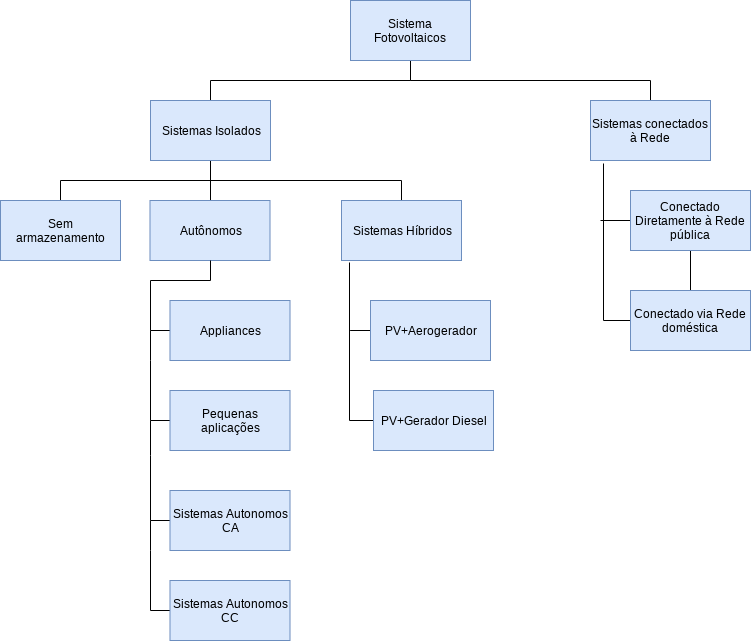
\includegraphics[width=1.0\textwidth]{figuras/sistemasFoto.png}
    \caption{Tipos de sistemas fotovoltaicos}
    \label{fig:caminho-objetos-scheduling}
\end{figure}

Um sistema fotovoltaico isolado não possui conexão com a rede de distribuição, podendo ser híbridos: quando existe a adição de outra fonte de energia, tais como geradores a combustível fóssil ou turbinas eólicas, ou autônomos, sendo esses constituídos apenas dos painéis solares. Já um sistema conectado à rede(\textit{On-Grid}) todo potencial gerado é escoado para a rede, sendo esses, mais eficientes que os sistemas autônomos, mesmo não tendo sistemas de armazenamento de energia, além de serem mais baratos.

Para utilizar um sistema fotovoltaico autônomo é necessário realizar um estudo sobre os equipamentos a serem utilizadas, suas demandas energéticas, quantidades, além de um estudo sobre quais os componentes que mais se adaptariam a tal projeto. Inicialmente deve-se calcular o gasto total diário baseando-se em quantos Watts/hora cada equipamento gasta e por quanto tempo ele será utilizado durante o dia. Para tal, podemos utilizar a seguinte fórmula:
% https://www.codecogs.com/latex/eqneditor.php?lang=pt-br
\[Consumo = \sum_{1}^{n}\left ( qtd.W \right )h\]

Onde temos que o consumo é proveniente da quantidade(\textit{qtd}) de equipamentos vezes a potência em \textit{Watts}(\textit{W})por hora vezes as horas(\textit{h}) de utilização. Em seguida, deve-se calcular a \textit{Potência instantânea} que o inversor de corrente deverá transferir as baterias, para isso, calcula-se a soma da potência dos equipamentos ligados simultaneamente.
\[Potência instantânea = \sum_{1}^{n} qtd.W  \]

Onde temos que o  potência instantânea é proveniente da quantidade(\textit{qtd}) de equipamentos vezes a potência em \textit{Watts}(\textit{W})por hora. Deve-se calcular uma folga para o inversor, tendo-se em mente que trabalham na faixa de 50\% e 70\% de sua capacidade, logo:
\[F_{max}=\frac{P.I}{0.5}\] e \[F_{min}=\frac{P.I}{0.7}\]

Dado os resultados, pode-se escolher um inversor autônomo que opere dentre essa faixa, tendo em vista a especificação de qual sua eficiência máxima, pois deve-se calcular o valor da energia gerada pelo sistema diariamente tendo-se em vista o autoconsumo do inversor:
\[ED =\frac{Consumo}{Eficiência Máxima}\]

A partir desses dados, é possível calcular a energia real da instalação:
\[ER=\frac{ED}{R}\]
Onde R é o Rendimento Global, calculado mediante fatores de perdas possíveis, normalmente assumindo o valor de 89\%(0,89). Por fim, calcula-se o valor da capacidade útil do banco de baterias, assumindo que \textbf{N} seja o valor de dias de autonomia do sistema e \textbf{Vi} sendo o valor da tensão
\[CU=\frac{ER*N}{Vi}\]
Vale a pena ressaltar que as baterias do sistema não podem ser descarregadas em sua totalidade, a carga real do sistema é dada por: 
\[CR=\frac{CU}{PD}\]
PD sendo o valor da profundidade da descarga da bateria. Por fim calcula-se o número de baterias a serem usadas, tanto em pararelo quanto em série:
\[NB=\left ( \frac{CR}{CN} \right )*\left ( \frac{Vi}{VB} \right )\]
Vb é a tensão nominal e CN a capacidade da bateria.

Em posse as características do sistema fotovoltaico idealizado e com os cálculos acima descritos, fica factível a construção de um sistema para suprir suas necessidades e respeitando as características dos seus componentes.

\section{Computação Autônoma}

Como sistemas tem se tornado cada vez mais interconectados e diversos, arquitetos estão cada vez menos capazes de antecipar e construir as interações entre os componentes, deixando esses problemas para serem resolvidos em tempo real. Logo, os sistemas ficaram gigantescos e muito complexos até mesmo para o mais qualificado dos integradores de sistema para instalar, configurar, otimizar, manutenir e conectar. A única opção restante é computação autônoma: sistemas que conseguem gerenciar a si mesmos dados certos objetivos\cite{Kephart2003}.

Um dos pilares essenciais de um sistema autônomo é a capacidade sensorial do mesmo, onde o habilita a observar o contexto externo. É também de suma importância que o sistema tenha propósito e \textit{know-how} para continuar operando sem ajuda externa, operação essa que é ditada pela lógica embutida responsável pelas tomadas de decisão para que o propósito e seus objetivos sejam alcançados, baseando-se também, no poder de interpretação dos dados provenientes dos sensores. Como é observado na Figura \ref{fig:modelo-conceitual}, o sistema deve ser capaz de produzir saídas, dado as entradas(objetivos, dados) e as informações provenientes dos sensores, tomando as corretas decisões e adaptando-se as mudanças de contexto.

\begin{figure}[H]
    \centering
    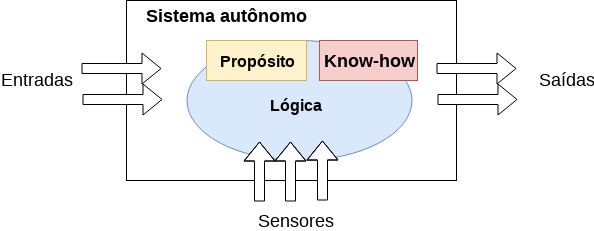
\includegraphics[width=0.7\textwidth]{figuras/autonomo.png}
    \caption{Modelo conceitual}
    \label{fig:modelo-conceitual}
\end{figure}


A essência de um sistema autônomo é o auto-gerenciamento, sendo este capaz de ajustar sua operação para comportar as mudanças de cargas de trabalho, demandas e condições externas, além de possíveis falhas de \textit{hardware} ou \textit{software}. O sistema deve ser capaz de compilar informações sobre uso de \textit{hardware}, desempenho dos \textit{softwares} e componentes a fim de ajudar em decisões futuras, sendo esses também, capazes de automaticamente reverter essas decisões se julgar que o resultado não mantenha ou melhore os padrões de disponibilidade do mesmo.

Sistemas autônomos são capazes de configurar-se automaticamente de acordo com as prioridades de alto nível que especificam o que é desejado do sistema. Ao incorporar novos componentes ao sistema, o mesmo deve se adaptar a adição, reconfigurando os demais componentes para que todos continuem a funcionar em sinergia. Além disso, esses sistemas devem, de forma continua, procurar modos de otimizar sua operação, buscando a melhor combinação de parâmetros e buscando a continua atualização dos componentes, isso, devido a grandiosa complexidade desses sistemas demandarem horas de trabalho de um especialista para que sejam otimizados.

A tarefa de encontrar um erro(\textit{bug}), descobrir suas causas e, por fim, construir uma solução pode consumir inúmeras horas de trabalho de uma equipe de programadores. Um sistema autônomo deve detectar, diagnosticar e resolver certos problemas que encontrar ou, se necessário, notificar os administradores do problema. O sistema é capaz de realizar tal tarefa, dado o conhecimento do próprio funcionamento e da performance que pode alcançar. Além disso, o sistema pode se proteger de ataques que possam acarretar perdas de performance e de disponibilidade, bem como utilizar seus sensores para verificar possíveis problemas e tomar decisões de como evita-los.

\section{Arduino}
Arduino é uma plataforma eletrônica de código aberto,  concebida para ser fácil de usar, tanto em termos de \textit{hardware}, como de \textit{software}. Por essa natureza, Arduino é indicado para \textit{hobbistas}\footnote{Segundo Corte Certo: Largamente em uso, vem do inglês hobbyist, nome que se dá a uma pessoa dedicada a um hobby.}, estudantes e professores, pois além de simples, é de baixo custo, multiplataforma e possui uma gama enorme de \textit{software} e \textit{hardware open-sorce}\cite{Mohammed2017}.

\begin{figure}[H]
    \centering
    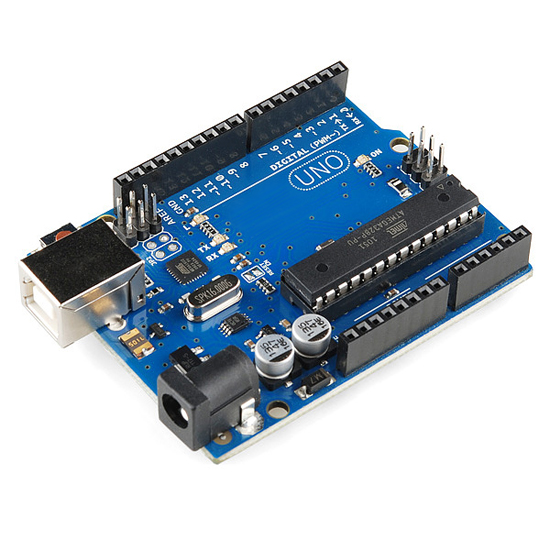
\includegraphics[width=0.7\textwidth]{figuras/Arduino_Uno_R3.png}
    \caption{Uma das várias versões do Arduino: a Uno R3}
    \label{fig:arduino-uno}
\end{figure}

A família Arduino é baseada no micro controlador ATmega32 de 8-bits, com \textit{clock} de 16mhz, várias entradas digitais e analógicas para IO, comunicação serial, USB e ICSP. Para sua operação, Arduino requer uma voltagem de 7 a 12V. Possui 35kb de memória, sendo essas: 32kb de memória \textit{flash}, onde os programas são carregados, 2kb de SRAM(\textit{static random access memory}) para manipulação de variáveis e \textit{erasable read only memory}(EEP-ROM) de 1kb  onde ficam os dados que devem ser persistidos. No site oficial do Arduino\footnote{https://www.arduino.cc/} encontra-se disponível também a IDE(\textit{Integrated Development Environment}) oficial, onde é possível editar e compilar códigos, bem como comunicar-se com a placa.

Um Arduino pode ser conectado a vários tipos de \textit{shields}\footnote{São placas de circuito que podem ser conectadas ao Arduino, encaixando-se perfeitamente por cima dele} para inúmeras aplicações, desde o controle de motores, módulos GPS, \textit{Wifi} e \textit{Bluetooth}. Por toda essa capacidade, Arduino vem crescendo dentro das indústrias também, onde um estudo feito por UBM\footnote{http://bd.eduweb.hhs.nl/es/2014-embedded-market-study-then-now-whats-next.pdf} em 2014, mostrou que 19\% dos profissionais questionados consideravam a utilização do Arduino nos próximos projetos.
\section{Raspberry PI}

Segundo o site do fabricante\footnote{https://www.raspberrypi.org/help/what-\%20is-a-raspberry-pi/} , Raspberry Pi é um computador de baixo custo, pequeno tamanho que pode ser conectado diretamente a um monitor ou aparelho de televisão. É capaz de rodar um sistema operacional, comumente o Raspbian, uma versão famoso sistema operacional Debian, criada especificamente para o Raspberry Pi. Apesar do pequeno tamanho, é possível executar tarefas de um computador normal, tais como programar, navegar na internet, assistir filmes em alta resolução, entre outros. 

A placa apresenta, na sua versão 2, um processador \textit{quad-core} de 900mhz  \textit{Broadcom} BCM2836 quad core Cortex A7, 1 GB de memória RAM, portas USB, Ethernet, cartão MicroSD, saía de áudio e HDM. Dadas essas características, essa versão é mais indicada a projetos que necessitem de mais processamento, muitas vezes usada como "cérebro" em projetos de Internet das Coisas.

\begin{figure}[H]
    \centering
    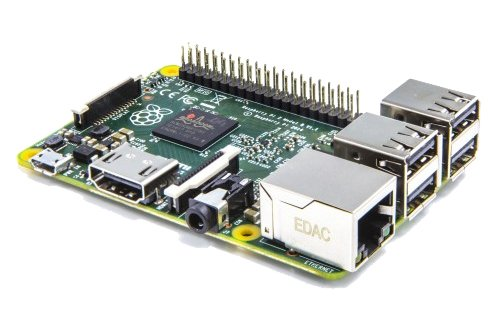
\includegraphics[width=0.7\textwidth]{figuras/raspberrypi2.jpg}
    \caption{Raspberry Pi 2}
    \label{fig:raspberry-pi}
\end{figure}

\section{Mapas georreferenciados}
Para \cite{Meng2014}, georreferenciamento é "alinhar dados geográficos com um sistema de coordenadas conhecidos para que possa ser pesquisado, visualizado e analisado com outros dados geográficos". O processo de identificar um objeto geográfico e relaciona-lo a uma locação geográfica é chamado de \textit{matching}\footnote{casar,igualar, combinar}. Georreferenciamento  normalmente usa um sistema de referencia chamado \textit{WGS-84}, que constrói coordenadas padronizadas para a terra, em adição, alguns dispositivos de navegação são utilizados para coletar dados e atrelá-los ao processo de construção do mapa. A combinação de dados provenientes de GPS em combinação com \textit{WGS-84}, podem referenciar a um certo ponto geográfico no mapa \ref{fig:mapa:georef}. Esse tipo de mapa pode combinar dados e imagens capturados por satélite, aeronaves ou veículos aéreos não tripulados. 

\begin{figure}[H]
    \centering
    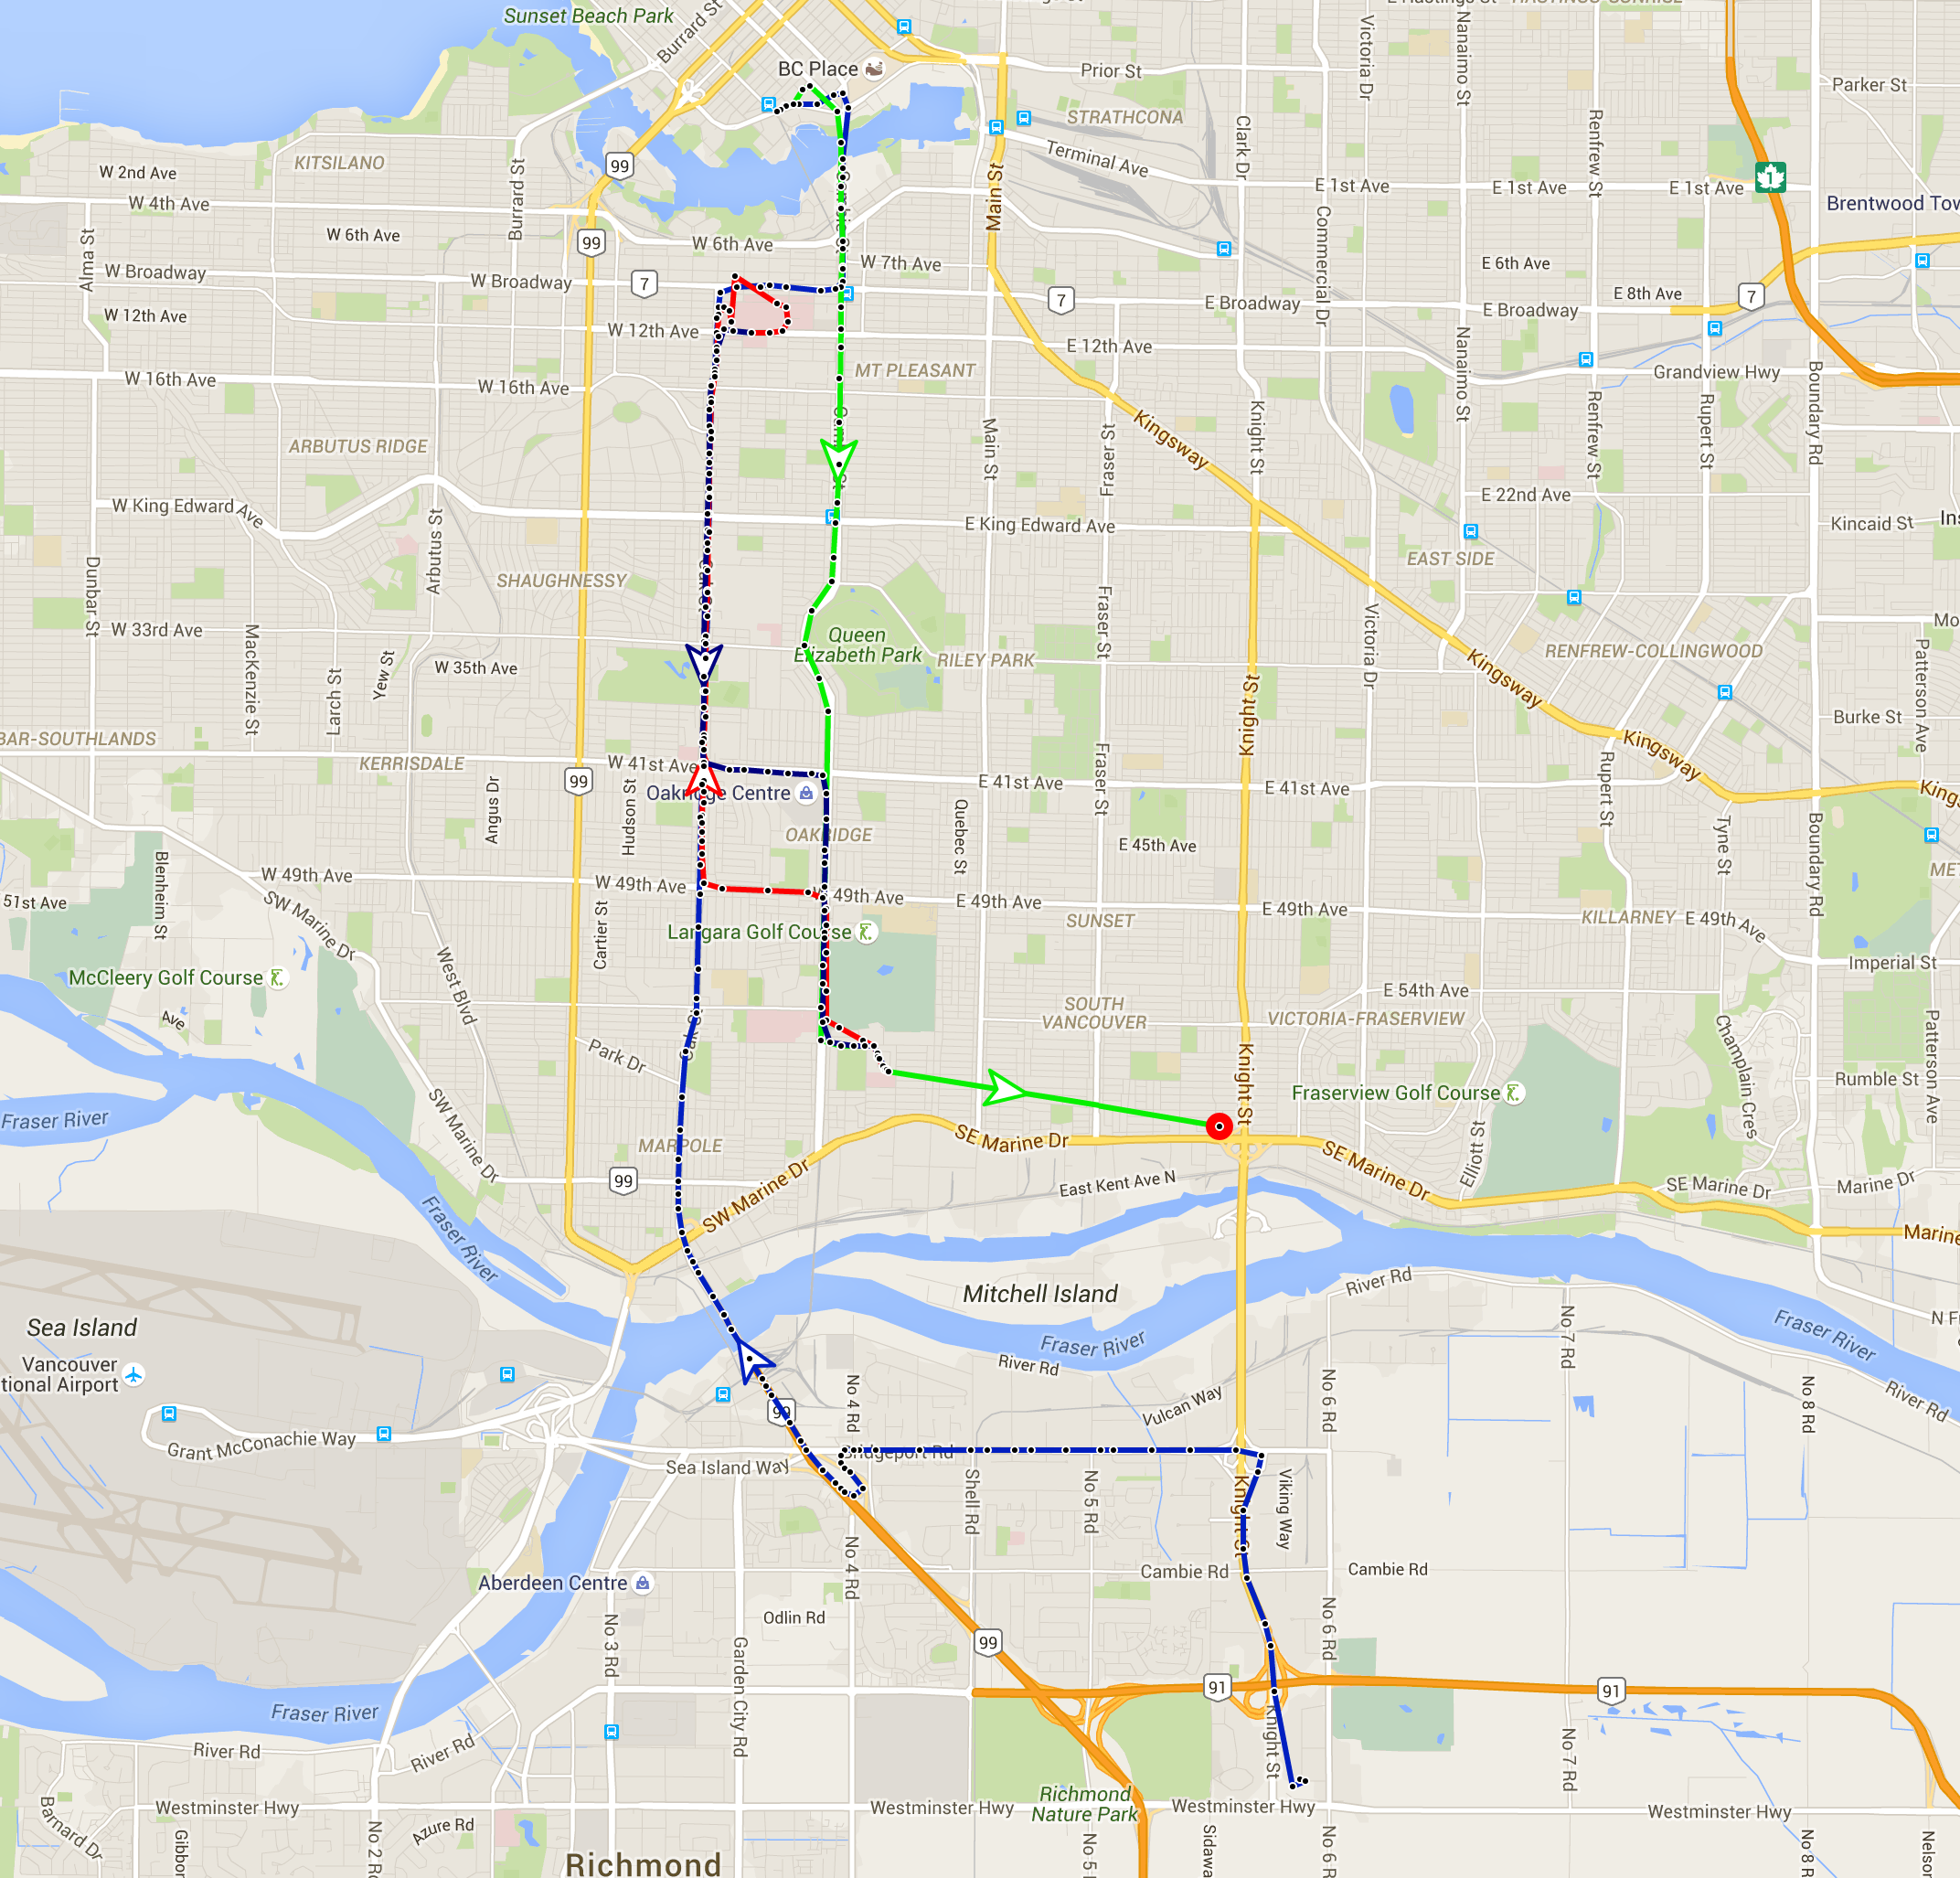
\includegraphics[width=0.7\textwidth]{figuras/Screen Shot 2016-05-12 at 3.25.21 PM.png}
    \caption{Mapa georreferenciado combinando dados de um GPS acoplado a um carro}
    \label{fig:mapa:georef}
\end{figure}

\section{Baterias}

%https://batteryuniversity.com/learn/archive/whats_the_best_battery

Uma bateria é um dispositivo com uma ou mais células eletroquímicas com conectores externos que conseguem prover eletricidade a outros dispositivos, tais como carros, computadores portáteis, celulares, entre outros. Alessandro Volta foi o primeiro a descrever uma bateria nos anos de 1800, onde através de uma pilha de zinco e cobre, separados por papeis enxercados com água salgada, produziu uma corrente estável por um considerável tempo. Atualmente existem inúmeros tipos de baterias, variando de tamanho, potência e composição, variando também pelo seu tempo de vida, capacidade de descarga e preço\cite{Buchmann2017}. Dentre as quais podemos citar:
\begin{itemize}
    \item \textbf{Níquel-cádmio(NiCd):} Um tipo já maduro na indústria, com pouca densidade energética, a bateria feita com NiCD é utilizada onde durabilidade, alta taxa de descarga e preço são importantes. Utilizadas em rádios, equipamentos biomédicos, câmeras de vídeo. Contudo, são tóxicas e nada amigáveis ao meio ambiente.
    \item \textbf{Hidreto de metal níquel(NiMH):} comparada com as baterias de NiCd, as de NiMH possuem maior densidade energética, mas com ciclo de vida menor. Contem metais tóxicos e são utilizadas em computadores e celulares.
    \item \textbf{Chumbo-ácido:} São as mais econômicas para utilização em grandes aplicações, onde o peso não é problema. São as mais utilizadas em equipamento hospitalar, cadeiras de roda e iluminação de emergência.
    \item \textbf{Íon de lítio(Li‑ion):} Vem crescendo em uso recentemente, já que podem ser utilizadas em aplicações onde peso e grande densidade enérgica são necessárias, na contramão, a tecnologia é frágil e precisa de proteção dos seus circuitos. Normalmente utilizadas em celulares e \textit{notebooks}.
    \item \textbf{Polímero de íon de lítio(Polímero Li‑ion): } São parecidas com as de Li-ion, mas mais finas e simplificadas, comumente usadas em telefones celulares.
\end{itemize}
 % Esse capítulo e nome é apenas uma sugestão.
\chapter{Histórico}
\label{cap:historico}
\section{Primórdios}
Veículos Terrestres não tripulados datam do inicio do século XX, onde em 1921 uma das primeiras aparições de um veículo desse tipo é relatada. A ideia inicial era de que a tecnologia poderia ser adaptada a tanques de guerra. O veiculo consistia de um chassi de 3 rodas com um motor e era controlado via rádio. Entre as décadas de 30 e 40, a União das Republicas Socialistas Soviéticas, bem como a Alemanha e o Reino Unido criaram versões e seus tanques operados remotamente, com os russos utilizando as suas versões no fronte contra a Finlândia.
\begin{figure}[!htb]
    \centering
    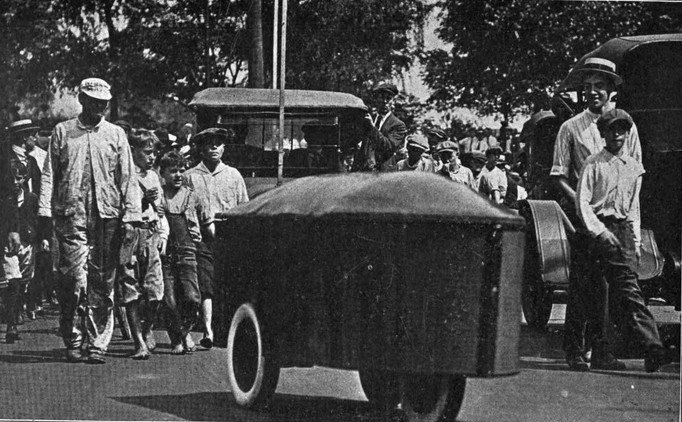
\includegraphics[width=0.75\textwidth]{figuras/controaldo_1921.jpg}
    \caption{Veículo controlado por radio em 1921}
    \label{fig:veiculo:1921}
\end{figure}

Ainda na década de 1940, os alemães criaram um pequeno veículo que utilizava lagartas para se mover para carregar explosivos até as posições inimigas. A inspiração veio de um projeto criado por Adolphe Kegresse encontrado depois da invasão a França. O projeto foi melhorado pelos alemães, recebendo o nome de \textit{Leichter Ladungsträger Goliath}, em português: carregador leve de carga Goliath. Esse pequeno veículo era capaz de carregar uma ogiva de 60kg de explosivos a uma distância de 650 metros. O controle era feito através de um cabo conectado a traseira do veiculo. 
\begin{figure}[!htb]
    \centering
    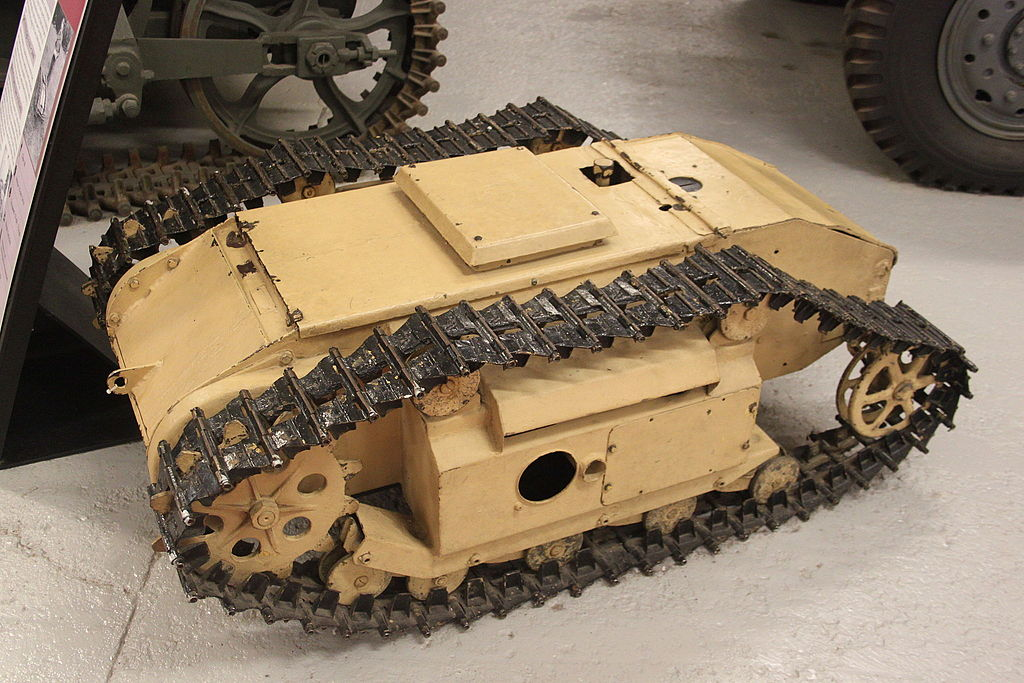
\includegraphics[width=0.75\textwidth]{figuras/goliath.JPG}
    \caption{Um exemplar do Goliath no museu de Tanques de Bovington}
    \label{fig:goliath:museu}
\end{figure}
Cerca de 7564 Goliaths foram construídos, contudo a utilização o mesmo foi limitado, dada a fragilidade do cabo de controle, além disso, a complexidade da sua manutenção no campo de batalha era grande, isso somadas a baixa velocidade, blindagem de apenas 10mm e o peso, considerado muito grande para ser facilmente transportado.
\section{Inicio da automação}
Na década de 60 surgiu o Shakey, o primeiro robô autônomo criado por Charles Rosen com fundos provenientes da Agência de Projetos de Pequisa Avançada de Defesa(Defense Advanced Research Projects Agency - D.A.R.P.A). Shakey conseguia perceber seus arredores e depois da análise do ambiente, criar um plano de ação para realizar um número de ações. 

\begin{figure}[H]
    \centering
    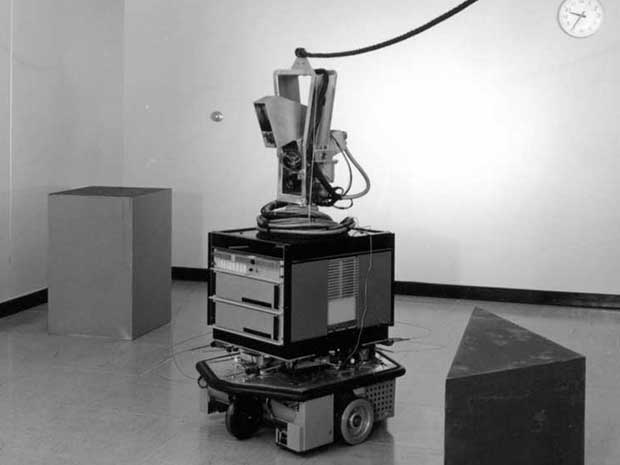
\includegraphics[width=0.75\textwidth]{figuras/shakey_robot.jpeg}
    \caption{Shakey, o robô. Seu nome vem do fato e chacoalhar muito durante sua movimentação}
    \label{fig:shakey:robo}
\end{figure}

A pesquisa de Shakey culminou em um grande impacto sentido em vários campos de pesquisa, tais como robótica e inteligência artificial, bem como a ciência da computação em si. A pesquisa resultou no algoritmo de pesquisa A* usado para achar caminhos e transversais de grafos. Além de avanços no processamento de imagens, visão computacional e análise de imagens.\cite{cassel:2017}

Já na década de 1970, a empresa Pyxus colocou no mercado o robô HelpMate desenhado a executar tarefas dentro de um hospital. Partindo do pressuposto de que tarefas de que "transporte" tomavam um tempo essencial dos enfermeiros e de que na época existia uma demanda desses profissionais, a ideia de criar um sistema que pudesse suprir essa demanda foi explorada. De forma autônoma, HelpMate, percorria o hospital mostrando um comportamento humanizado carregando refeições, suprimentos estéreis, medicações, registros médicos, amostras e cartas.\cite{evans:1992}. Ele conseguia se movimentar pelo hospital graças a mapas pré-carregados em seu sistema. Além disso, era dotado de sonares, infravermelho e detectores de colisão.
\begin{figure}[H]
    \centering
    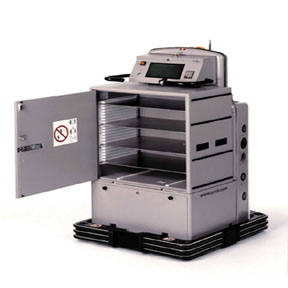
\includegraphics[width=0.75\textwidth]{figuras/helpmate.jpg}
    \caption{HelpMate, robô para auxiliar em atividades de transporte em hospitais}
    \label{fig:helpmate:robo}
\end{figure}

HelpMate conseguia 98\% de sucesso em suas missões, logando em seus sistemas os sucessos e também os  motivos por uma possível falha. Ficou claro que as falhas catalogadas eram provenientes de erros do usuário ou de forças externas a suas capacidades, como tarefas agendadas de forma errônea, falhas em elevadores ou paradas emergências e não por falhas de hardware ou incapacidade de navegar até seus objetivos.

A CyberMotion criou por sua vez o SR2, um robô de 3 rodas para segurança de instalações equipado com um sistema e navegação ultrassônico e um sistema anticolisão, além disso, era equipado com sensores de umidade, fogo, fumaça ou gases, podia detectar movimento e avisar caso percebesse um intruso. Contudo, a empresa falhou em fazer o produto vender, fechando as portas em 2005\cite{bracht:2015}.
\begin{figure}[H]
    \centering
    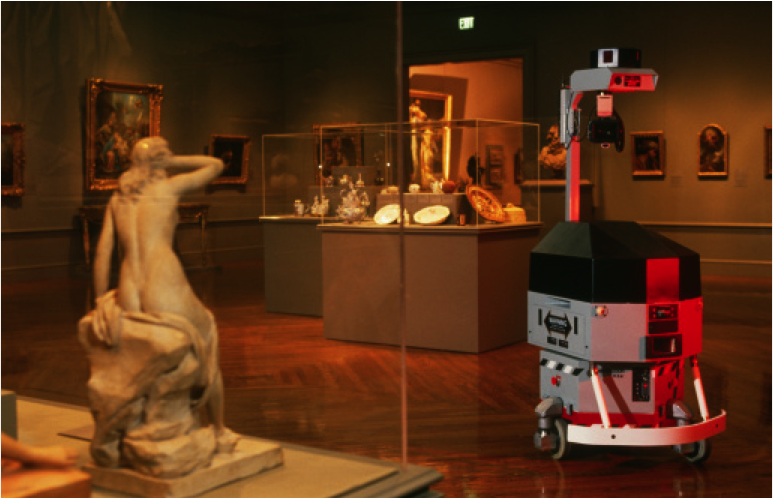
\includegraphics[width=0.75\textwidth]{figuras/cybermotion SR2.png}
    \caption{Robô de segurança SR2 da CyberMotion}
    \label{fig:cybermotion:sr2}
\end{figure}


\section{Aplicação na agricultura}
Em 2016 na \textit{Farm Progress Show} no estado de Iowa foram apresentados pela \textit{CNH Industrial} dois protótipos de tratores autônomos: o \textit{Case IH Magnum} e o \textit{New Holland T8 NHDrive}. Apesar de tecnologias capazes de controlar certos aspectos da operação de um trator já existirem, como direção automática e correção de direção por GPS, as empresas foram além, criando sistemas autônomos capazes de operar por completo os tratores. Já que são baseados em tratores já existentes, a maioria de componentes convencionais foram mantidos como motores, transmissões, chassi e módulos de acoplagem e no caso do \textit{T8 NHDrive}, a cabine do operador foi mantida por questões operacionais.\cite{engineer:2016}

A \textit{Jacto} por sua vez vem trabalhando no seu próprio veiculo aqui no Brasil, o \textit{Jacto Autonomous Vehicle}, desde 2008. O \textit{JAV} é capaz de operar na lavoura por horas sem intervenção humana, sendo capaz também de trocar informações e dividir o trabalho entre outros veículos que estejam na mesma área.\cite{jacto:2018} Até o momento o JAV é apresentado na versão de pulverização, mas os projetos podem ser modificados no futuro para que possa receber outras funções.

\begin{figure}[H]
    \begin{center}
    % jacto
        \subfigure[]{
            \label{Jacto:jav}
            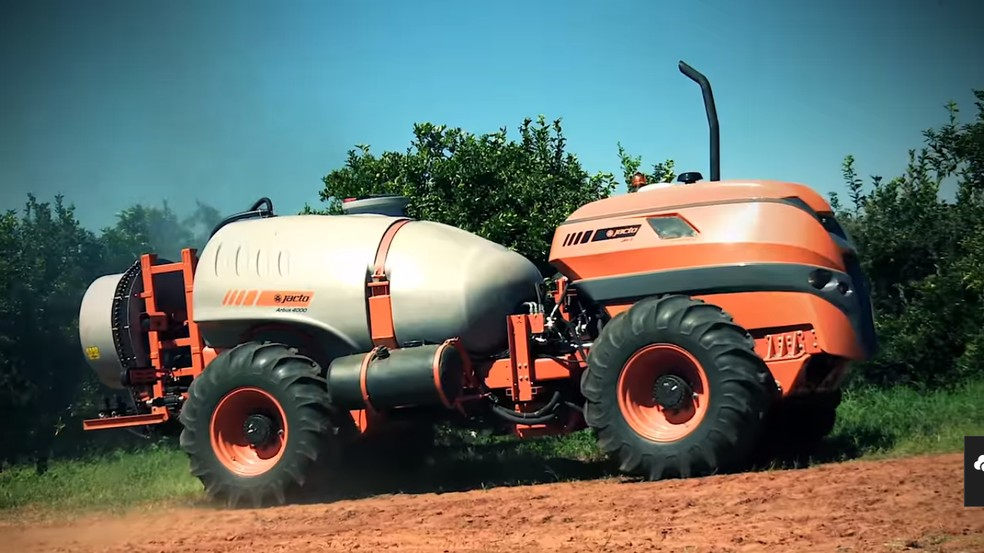
\includegraphics[width=0.4\textwidth]{figuras/jacto-jav.png}
        }
        % new holland
        \subfigure[]{
            \label{Holland:T8}
            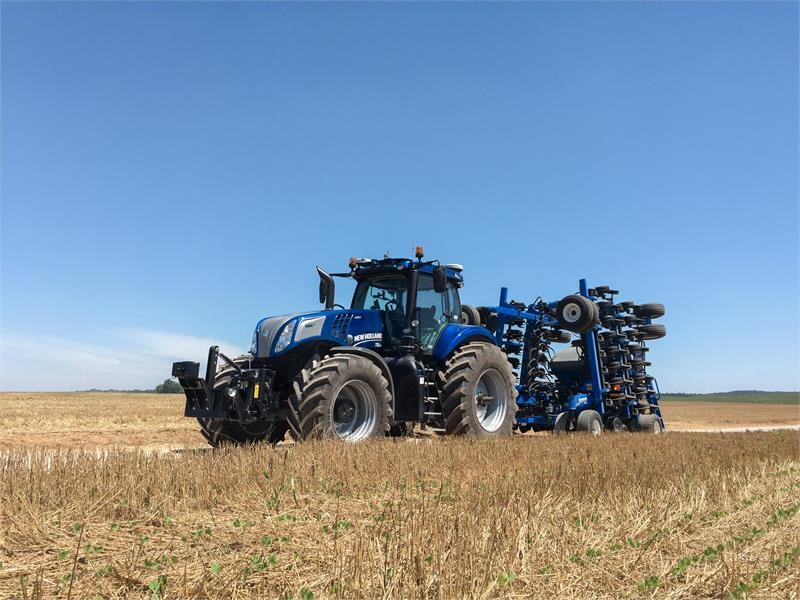
\includegraphics[width=0.4\textwidth]{figuras/newhollandt8.png}
        }
           % CASE
        \subfigure[]{
            \label{Case:Magnum}
            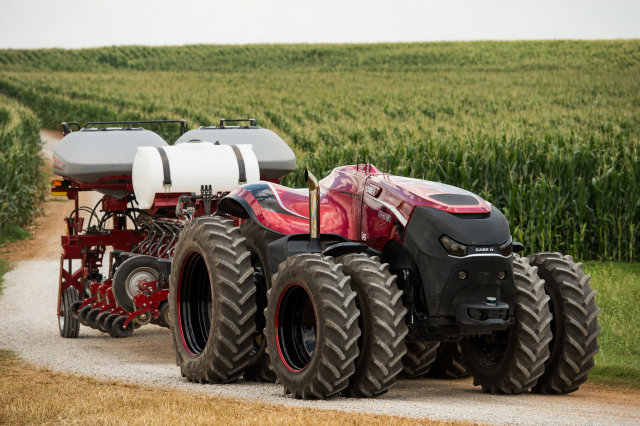
\includegraphics[width=0.4\textwidth]{figuras/CaseMagnum.jpg}
        }
    \end{center}
    \caption{%
        (a) Jacto JAV II, (b) New Hollando T8 NHDrive, (c) Case IH Magnum
     }%
\end{figure}


Os três veículos, apesar de implementados de forma diferente, operam similarmente: um plano de trabalho é criado baseado em uma área pré-estabelecida através de coordenadas GPS, após isso, um sistema calcula a melhor rota a ser seguida, levando em consideração consumo de combustível, obstáculos, o tamanho dos implementos agrícolas\footnote{Implementos agrícolas são apetrechos que são necessários para desempenhar uma certa ação. Exemplo: arados, plantadoras, niveladoras} acoplados e outras máquinas operando na vizinhança. Caminhos podem ser inseridos manualmente caso seja necessário. Todo esse sistema pode ser controlado via dispositivo móvel ou em um computador, onde também serão mostrados os caminhos a serem tomados, bem como o progresso da operação, além de opções para modificação dos parâmetros de operação dos implementos.

Para tais missões, as máquinas são dotadas dos mais diversos sensores, passando de várias câmeras, microfones, sensores de proximidade e até mesmo radares. Com esse vasto arsenal possibilita-se que o sistema tome decisões durante sua missão, tais como evitar obstáculos ou colisões. Dado o nível de autonomia das mesmas é possível que um operador seja capaz de gerenciar N veículos com diferentes funções, acompanhando o progresso de cada uma e ajustando os parâmetros se necessário.

% ATENÇÃO - veja com o seu orientador se você vai ter este capítulo e se este vai ter nome!
\chapter{Trabalhos Relacionados}
\label{cap:trabalhos:relacionados}
Com a crescente necessidade de alcançar maiores níveis de produtividade e escassez de mão de obra tanto capacitada como a não capacitada, a indústria agrícola vem buscando novos meios de atender as demandas atuais. Combinando automação com agricultura de precisão, busca-se aumentar a produtividade e diminuir a dependência por mão de obra no campo. Para tal, várias frentes de pesquisas vem sendo abertas tanto por universidades, bem como grandes indústrias. 

\section{Projeto de um veículo Autônomo capaz de cobrir um área poligonal sem passar mais de uma vez pela mesma região}
No trabalho desenvolvido por \cite{bracht:2015} foi desenvolvido um sistema de pilotagem para veículos agrícolas, que de forma autônoma fossem capazes de exercer a função de espalhadores de produtos agrícolas, tais como herbicidas ou estimulantes, tendo-se em vista a necessidade do mesmo não passar pela mesma área mais de uma vez, evitando-se desperdício, danos por quantidades acima do ideal e até mesmo impactos ambientais.

Dadas as limitações causadas por veículos articulados comumente usados na agricultura, foi concebido um robô para fins experimentais de corpo único, constituído por 3 rodas: duas ligadas a motores e uma roda direcional responsável pela sustentação. Esse tipo de montagem, como pode ser observado na Figura \ref{fig:chassi:robo}, facilita a construção devido ao número reduzido de peças necessárias.
\begin{figure}[H]
    \centering
    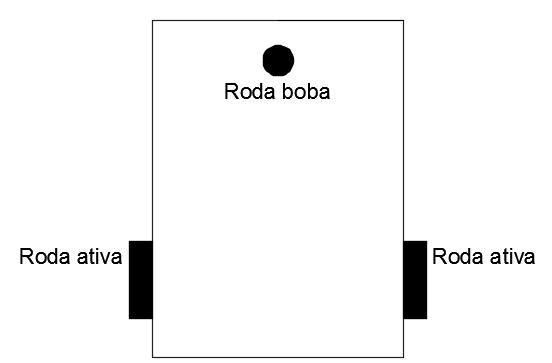
\includegraphics[width=0.75\textwidth]{figuras/robo bach.png}
    \caption{Esquema do chassi proposto}
    \label{fig:chassi:robo}
\end{figure}
Para controle direcional utilizando os dois motores acoplados as rodas, foram criados modelos matemáticos que possibilitam calcular a rotação do robô tendo em vista a velocidade angular das rodas.

O algoritmo usado neste trabalho consiste em transformar o polígono descrito em uma matriz de números, onde 1's representam a área do polígono Figura \ref{fig:matriz:poligono}. A escolha da melhor trajetória consiste em um problema de minimização de uma função-custo.
\begin{figure}[H]
    \centering
    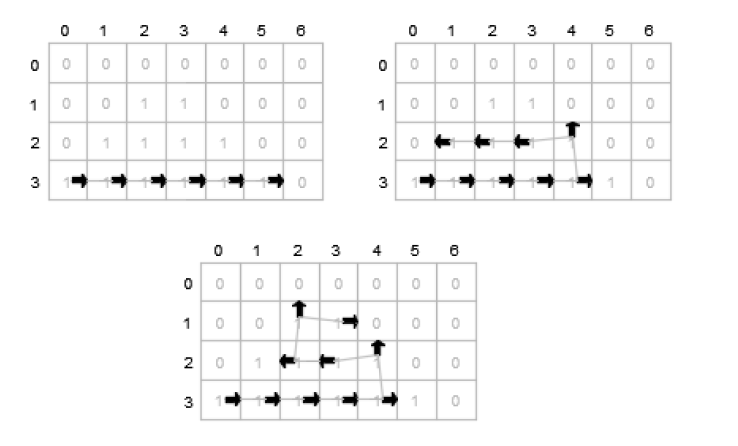
\includegraphics[width=0.75\textwidth]{figuras/matrizesPoligno.png}
    \caption{Matrizes poligonais}
    \label{fig:matriz:poligono}
\end{figure}
\section{Autonomous Maneuvers of a Robotic Tractor for
Farming}

Com objetivo de diminuir a carga de trabalho dos trabalhadores rurais, a solução apresentada por \cite{Wang2016} aborda o controle de manobras para um trator de 4 rodas feito para trabalhar em plantações enfileiradas, bem como testes feitos em tipos diferentes de solo para avaliar a performance do mesmo.

O sistema foi construído utilizando um trator do modelo EG105 fabricado pela \textit{YANMAR} \ref{fig:yanmar:eg105} no Japão, além de servos para controlar os ângulos de direção do mesmo. Para um posicionamento mais refinado do trator, utilizaram-se ainda um \textit{Real Time Kinematic Global Positioning System} (RTK-GPS) com a adição de dados de correção oriundas de uma rede chamada \texit{GPS Earth Observation Network}(GEONET)  disponível no Japão. 

\begin{figure}[H]
    \centering
    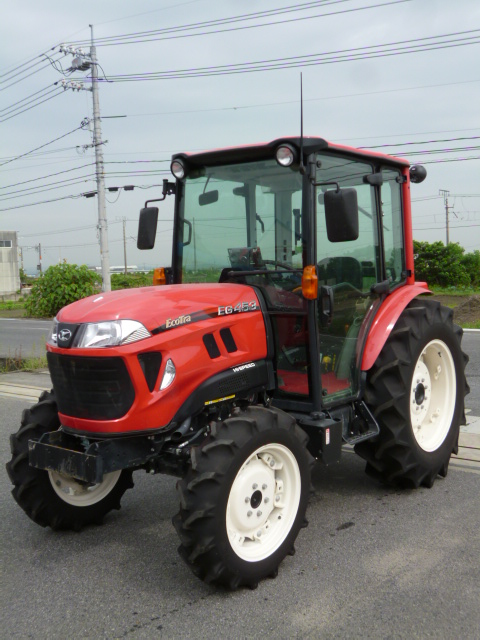
\includegraphics[width=0.55\textwidth]{figuras/EG105 yanmar.JPG}
    \caption{Yanmar EG105}
    \label{fig:yanmar:eg105}
\end{figure}

As manobras do trator foram programadas para imitar as manobras realizadas por operadores humanos, baseadas em arcos e círculos e seguimentos de reta. A direção desejada era determinada pela posição atual do trator e a posição de um ponto de navegação, os ângulos de curva são calculados baseados na diferença lateral e de direção do mesmo.

O sistema foi avaliado quanto a sua performance resultando em erros máximos de 10 centímetros entre a posição real do trator e a traçada pelos algoritmos, sendo que a diferença entre o vetor de direção real e o programado não passaram de 3º, provando que o mesmo pode operar de forma precisa sem necessidade de grandes mudanças de direção. Com esses resultados foi concluído que o robô trator pode operar autonomamente a 5km/h com erros aproximados de 6cm em relação a sua posição e 1.2º em relação ao vetor de direção.
\section{Path Planning Mobile Robot Using Waypoint
For Gas Level Mapping}

Dada a alta periculosidade envolvida na detecção de gases tóxicos, tanto de origem natural, bem como de origem da ação humana, cresceu a necessidade de automatizar os meios de detecção destes. Pensando nisso, foi desenvolvido um robô capaz de detectar gases tóxicos e se locomover seguindo pontos pré-estabelecidos, a fim de minimizar o possível contato humano com situações adversas à saúde.  Composto por quatro rodas e com sensores para detecção de gases, o robô foi montado sob um chassi de 4 rodas independentes como visto na \ref{fig:gas:chassi}. Para localização foram utilizados um GPS e compassos.
\begin{figure}[H]
    \centering
    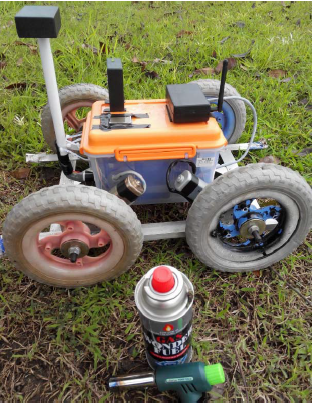
\includegraphics[width=0.55\textwidth]{figuras/chassi_robo_gas.png}
    \caption{Robô móvel utilizado}
    \label{fig:gas:chassi}
\end{figure}
A técnica utilizada para direcionar o robô foi baseada na premissa de que todas as rodas giram na mesma velocidade, logo, ao aumentar a velocidade de giro de uma delas, é mudada a direção do robô. Para direção, foram feitos cálculos baseados na posição atual do robô e a posição o próximo \textit{waypoint} e a diferença entre a direção do robô e a direção do \textit{waypoint}. Depois disso, era calculada a distancia até o \textit{waypoint} usando a fórmula de Pitágoras. Durante a movimentação até o \textit{waypoint}, dados são coletados tanto do GPS quanto do sensor de gases e enviados ao servidor através de um rádio.

Uma interface foi criada por \cite{Watiasih2017} onde pode-se ver os \textit{waypoints} e os pontos de presença de gases, além da leitura o sensor em tempo real. Nessa interface, apresentada na Figura \ref{fig:gas:interface}, é possível também inserir os \textit{waypoints} a serem seguidos, tendo esses um número máximo de 100 para que não excedesse a capacidade de memória do robô.
\begin{figure}[H]
    \centering
    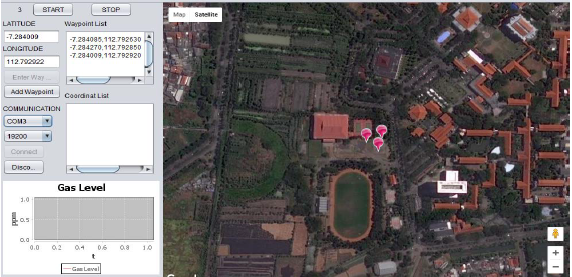
\includegraphics[width=0.7\textwidth]{figuras/interface_robo_gas.png}
    \caption{A interface conta com um mapa e caixas de textos para a inserção dos \textit{waypoints}}
    \label{fig:gas:interface}
\end{figure}
Testes levaram a um acerto de 95\% em relação a direção o robô e um erro de 3 metros em relação a posição real do \textit{waypoint}. Acredita-se que o número de satélites ao qual o GPS estiver travado interfira diretamente na precisão do mesmo.
\section{Scheduling and Control of Unmanned Ground Vehicles for Precision Farming: A Real-time Navigation Tool}

Este trabalho tem como objetivo a apresentação de um sistema para controle e agendamento  e veículos agrícolas autônomos(VAA) com objetivo de executar agricultura de precisão de forma ótimo. \cite{vlachos:2017} cara a hipótese elementar do trabalho dita que um campo e agricultura apresentam obstáculos, tanto aleatórios como estáticos, que um VAA deve detectar e recalcular seu caminho ótimo.  A grande contribuição deste trabalho vem da proposta de uma ferramenta de  \textit{software} em tempo real que reconheça o campo e guie o veículo para suas tarefas enquanto proporcione um melhor uso dos recursos e, potencialmente, uma melhor colheita.

O sistema proposto visa navegar o VAA pelo campo para realizar tarefas de precisão, tais como fertilização, pulverização e plantio, para tal, ele é dividido em quatro partes: uma camada representando a paisagem; uma camada representando os objetos estáticos. Tais como árvores e pedras; uma camada representando os agentes de ação(VAA); uma camada representando as mensagens trocadas entre o nós do sistema e por fim uma camada que trata todas as informações , que prioriza e otimiza os caminhos do(s) VAA(s) no campo. Na questão do campo em si, são necessário dados sobre as fronteiras do campo, informações sobre potenciais obstáculos e a direção dos caminhos presentes no campo, bem como o \textit{layout} das plantações. São determinadas também as características quanto a tamanho do VAA afim o sistema conseguir calcular distância seguras entre o mesmo e as plantações e/ou obstáculos. Com todas essas informações carregadas, bem como o \textit{feed-back} dos sensores presentes no VAA, o sistema é capaz de gerar um mapa e os caminhos a serem seguidos, como visto na Figura \ref{fig:caminho-objetos-scheduling}, onde observa-se a disposição os objetos, bem como o caminho o VAA. 
\begin{figure}[H]
    \centering
    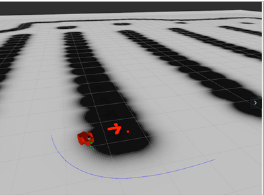
\includegraphics[width=0.7\textwidth]{figuras/caminho-objetos-scheduling.png}
    \caption{Representação gráfica dos dados disponíveis pelo sistema}
    \label{fig:caminho-objetos-scheduling}
\end{figure}

Os resultados comprovam a eficácia de tal abordagem, visto que com a adição dos sensores presentes no VAA, tais como o LiDAR(\textit{ Light Detection And Ranging}) que escaneia os arredores do VAA na busca por possíveis colisões, o mesmo consegue passar pela plantação com extrema precisão, possibilitando a utilização do mesmo em plantio em filas.
 % Esse capítulo e nome é apenas uma sugestão.
% ATENÇÃO - veja com o seu orientador se você vai ter este capítulo e se este vai ter nome!
\chapter{Proposta}
\label{cap:proposta}

O êxodo rural corresponde ao processo de migração em massa da população de campo para as cidades, fenômeno que costuma acontecer em períodos de tempo considerados curtos, com prazo de algumas décadas. Trata-se de um elemento diretamente associado a várias dinâmicas socioespaciais, tais como a urbanização, a industrialização, a concentração fundiária e a mecanização do campo.\cite{Pena2013}

Nos períodos de entre 1950 e 1980 o êxodo rural brasileiro chegou ao seu pico onde aproximadamente 30\% da população rural migraram para as cidades. Na ultima década, a migração perdeu velocidade, mas continuou a representar uma grande mudança no ambiente rural, onde 5,6 milhões de pessoas, 17,6\% da população rural, mudou-se para a cidade.\cite{Marra2011}

Os motivos para tal ocorrência são inúmeros, dentre eles: melhores condições de vida na cidade, o fim de unidades de produção familiares compradas por grandes latifundiários, queda na fecundidade e massiva mecanização das operações agrícolas.

Com enxada, foice e demais ferramentas, uma família não é capaz de cultivar três de acres de terra. Essa é uma das razões pelas quais tanto os agricultores familiares quanto assentados pedem veementemente para o governo para linhas de créditos a fim de se adequar a corrente de mecanização. \cite{Alves2013}

As máquinas e os equipamentos são indispensáveis para se realizarem tarefas dentro de um calendário ótimo e de acordo com as exigências de qualidade e do clima. Dão conforto aos trabalhadores e protegem sua saúde na aplicação de agrotóxicos, por exemplo. No caso de grãos, sem as plantadeiras de alta precisão, não se obtêm níveis remuneradores de produtividade. As colheitadeiras permitem realizar as tarefas num calendário compatível com as exigências dos mercados interno e externo. Na produção de leite, a ordenhadeira é fundamental para se obter nível de qualidade exigido e é importante para se obter o nível de qualidade exigido e é importante para reduzir o esforço dos trabalhadores. O Brasil dispõe de vastas áreas, dentro da fronteira agrícola já ocupada e em termos de terras degradadas, para se incorporarem à agricultura comercial. Pelos métodos manuais, tal incorporação é impossível, tanto tecnicamente como também porque grande parte da população foi drenada para as cidades. Assim a expansão da agricultura requer a mecanização.

A agricultura de precisão e uma filosofia de gerenciamento agrícola que parte de informações exatas, precisas e se completa com decisões exatas. Agricultura de precisão, também chamada de AP, é uma maneira de gerir um campo produtivo metro a metro, levando em conta o fato de que cada pedaço da fazenda tem propriedades diferentes.\cite{Tschiedel2002}

A agricultura de precisão é um sistema de manejo de produção integrado, que tenta igualar o tipo e a quantia de insumos que entram na propriedade com as necessidades da cultura em pequenas áreas dentro de um campo da propriedade. Para tal, essa filosofia anda de mão dadas com outras tecnologias: sensoriamento remoto, sistemas de informações geográficas(SIG) e de posicionamento global(GSP). A junção das tecnologias com esse tipo de pensamento pode vir a reduzir riscos nas atividades agrícolas, reduzir custo, ajudar na tomada de decisões, maior produtividade e menor impacto ambiental.
%apresentar a ideia
Com advento da mecanização agrária, da agricultura de precisão e da constante diminuição da população rural, consequentemente, da mão de obra, a automação do campo vem como ideia plausível e factível de como resolver e incorporar tais aspectos nos próximos anos na já industrializada produção do campo. Tendo em vista os vários frontes de pesquisa na área da automação agrária, é concebível a criação de um veículo autônomo terrestre que possa exercer certas funções no campo sem a interferência humana. 

Para tal, é necessário um algoritmo robusto, capaz de interpretar os dados dos sensores, bem como dados do GPS, combinando-os com mapas georreferenciados para que possa traçar um caminho seguro, seja ele de translado ou mesmo durante as tarefas no campo \ref{fig:entrada:saida}. O algoritmo deve ser capaz de, mediante obstáculos, recalcular sua rota, evitando o obstáculo e continuar seu trabalho, evitando danos ao próprio veiculo, a outros veículos ou até mesmo pessoas. Em adição, o algoritmo deve ser capaz de saber sua localização em relação a área de operação, tomando decisões de como atingi-la com certo nível de precisão. Em relação a área e operação, o veículo deve ser capaz de navegar por toda a área sem passar pelo mesmo caminho, evitando desperdício de recursos e de tempo.

\begin{figure}[H]
    \centering
    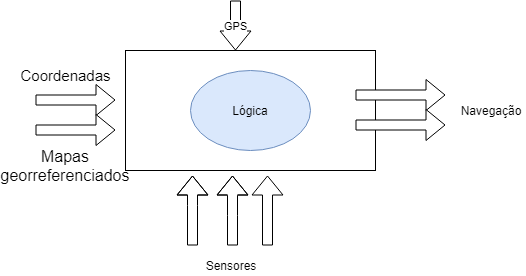
\includegraphics[width=0.75\textwidth]{figuras/entradaSaida.png}
    \caption{Conceito do algoritmo}
    \label{fig:entrada:saida}
\end{figure}

O algoritmo deve, de forma constante, medir a distância entre o seu ponto de destino e sua posição atual, ao mesmo tempo em que verifica sua atual direção e compara com a direção do ponto de destino. Em paralelo a isso, os sensores de distância devem ser lidos ininterruptamente em busca de possíveis obstáculos, evitando possíveis colisões. 
\begin{figure}[H]
    \begin{center}
    
        \subfigure[]{
            \label{fig:distância:alvo}
            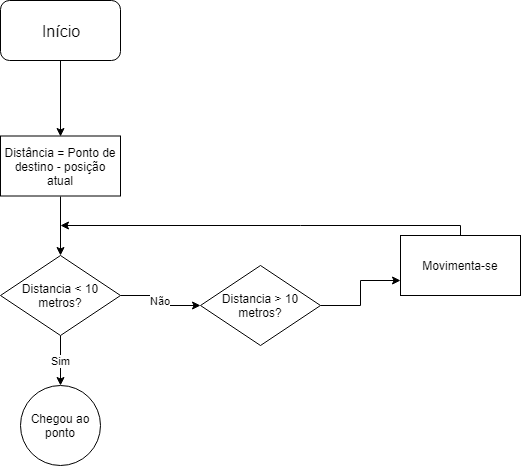
\includegraphics[width=0.4\textwidth]{figuras/ManicaDeEstados.png}
        }
        
        \subfigure[]{
            \label{fig:obstaculos}
            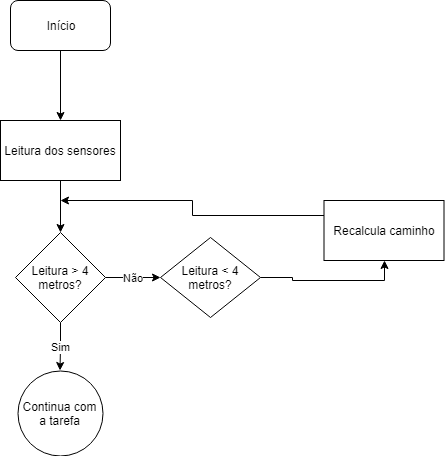
\includegraphics[width=0.4\textwidth]{figuras/obstaculos.png}
        }
      
    \end{center}
    \caption{%
        (a) Distância entre os pontos, (b)Evitar os obstáculos
     }%
\end{figure}



A ideia da criação de um veículo dessa categoria une a mecanização com a agricultura de precisão, tendo em vista a união dos dois mundos na criação de um equipamento que possa, através de sensores, compreender o ambiente ao seu redor, bem como combinar dados provenientes de GPSs para que se situe dentro de uma área pré-estabelecida e possa, com segurança, exercer suas funções durantes horas, quiçá dias, dadas boas condições de operação. O Brasil é um país de dimensões continentais do clima variando entre o equatorial até o semiárido com grande incidência de raios solares e combinando isso ao ambiente de operação, a utilização de fontes de energia provenientes da luz solar se torna interessante e implementável.

Em essência a utilização de sistemas fotovoltaicos, combinados a algoritmos de melhor caminho, sensores de distância, GPSs e um sistema de monitoramento que possa acompanhar o desempenho do veículo no campo, assim como em \textbf{4.3}, pode vir a culminar em um veículo terrestre de médio porte capaz de pulverizar, semear ou coletar informações sobre o campo.

A proposta a ser descrita idealiza um veículo de 4 rodas, movido por um único motor elétrico, sensores de ultrassônicos de distância, GPS e luzes, bem como painéis fotovoltaicos para produção de energia. A utilização de lagartas mecânicas foi descartada dada a complexidade da manutenção, a possibilidade de durante uma curva, uma das lagartas sair dos trilhos causando danos a suspensão e imobilizando o veiculo, bem como os danos causados ao solo. 

A figura \ref{fig:sketchup:vaa} apresenta uma visão geral do veículo, onde observa-se a maioria dos componentes externos: GPS, painel fotovoltaico e os sensores ultrassônicos. Logo abaixo do apoio superior, ficaram os demais componentes, tais como Arduinos, Pontes H, o \textit{shield} do GPS e outros servos. 
\begin{figure}[H]
    \centering
    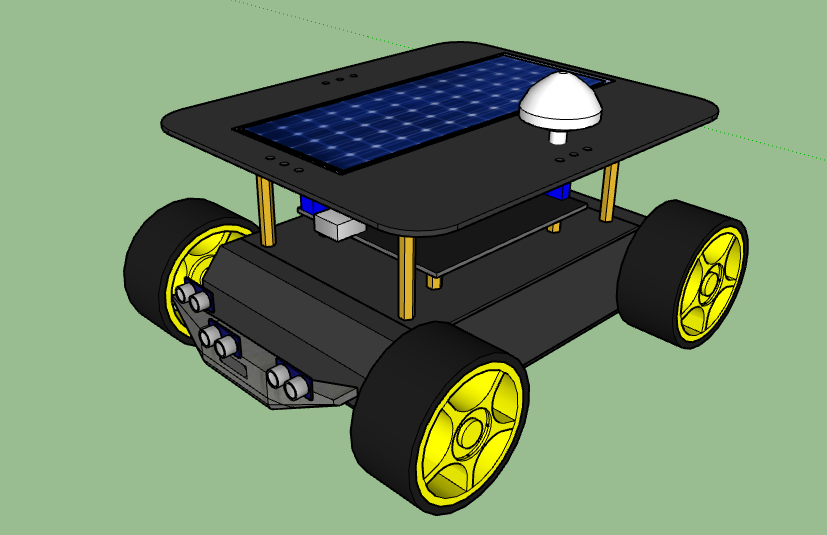
\includegraphics[width=0.75\textwidth]{figuras/chassi_vaa_completo.png}
    \caption{Esquema do chassi feito no Sketchup}
    \label{fig:sketchup:vaa}
\end{figure}
O veículo apresentado na figura \ref{fig:sketchup:vaa} sofrerá revisões ao longo do trabalho, principalmente em relação ao seu chassi, dado a necessidade de uma altura maior e espaço entre rodas. Contudo, a parte superior deve continuar nesse \textit{layout}.
O veículo possuirá, inicialmente, 3 sensores ultrassônicos dispostos na frente do mesmo, afim de captar possíveis obstáculos em sua rota, fazendo com o veiculo seja capaz de realizar manobras para evitar colisões e manter-se em distância segura das plantas do campo. Na figura \ref{fig:ultrasonico:vaa} podemos observar o esquemático gerado no Fritzing\footnote{http://fritzing.org/home/} representando um Arduino UNO R3 e 3 sensores ultrassônicos HCSR05.
\begin{figure}[H]
    \centering
    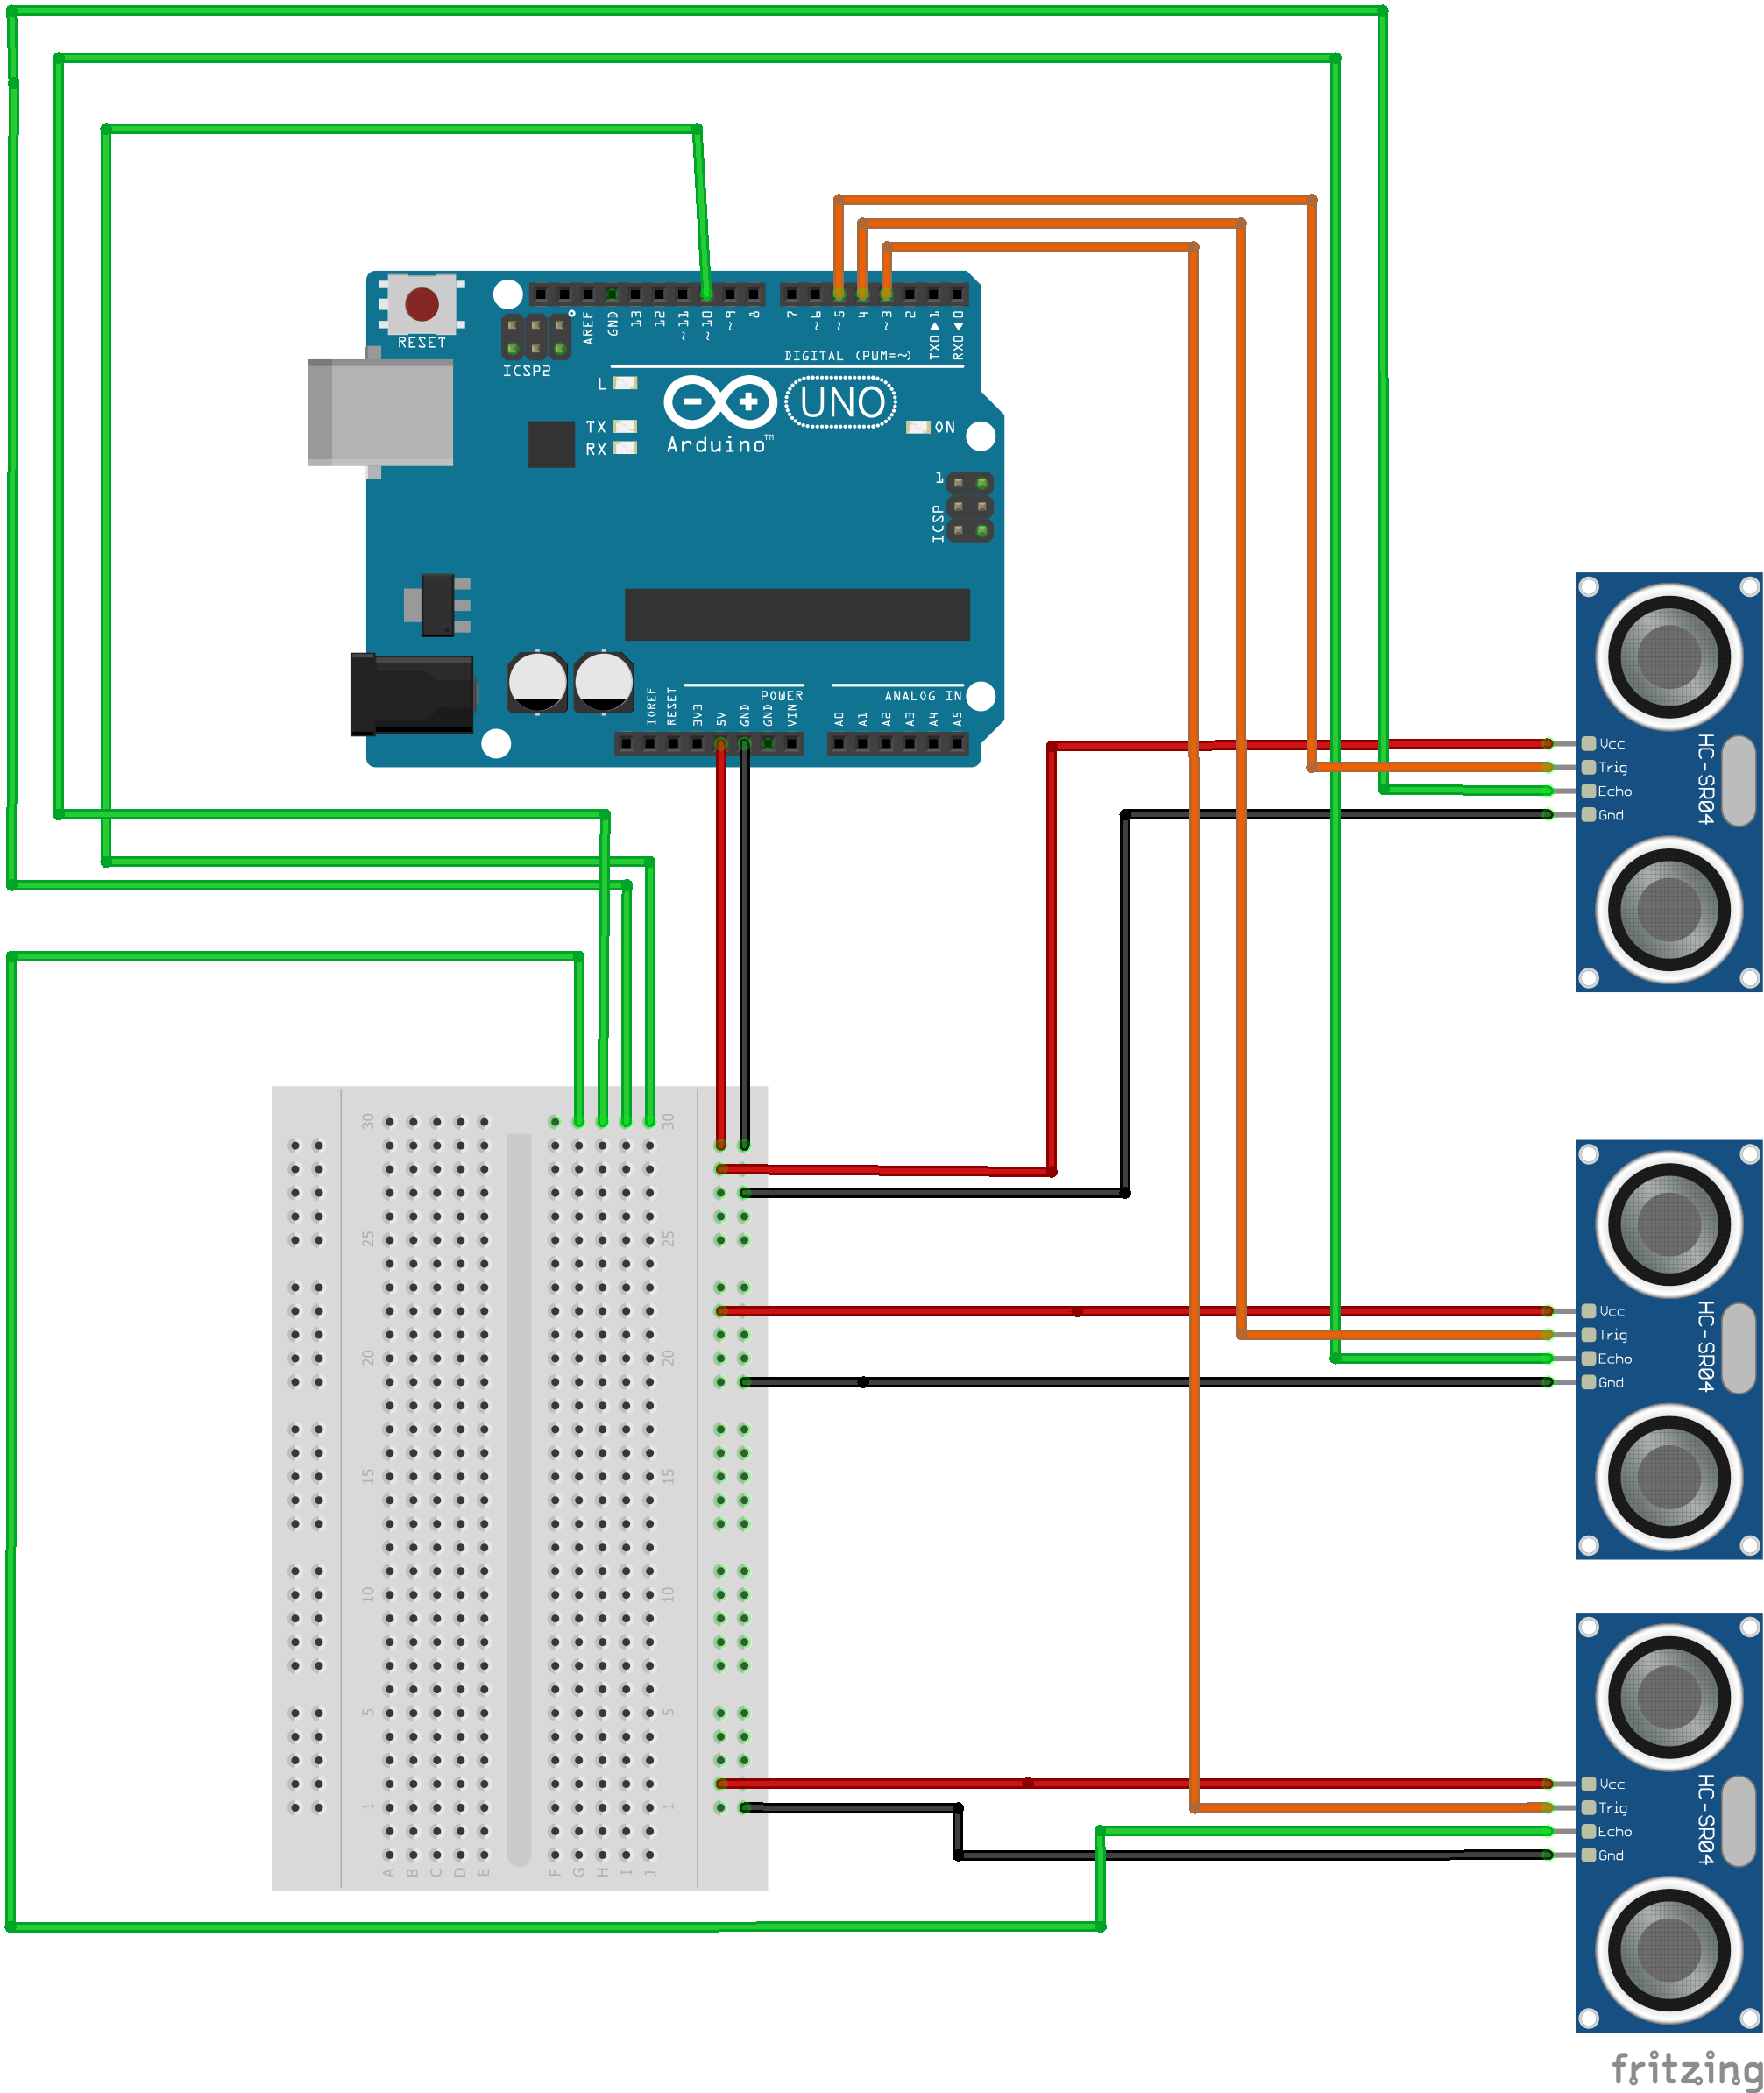
\includegraphics[width=0.5\textwidth]{figuras/ultrassonico_bb.png}
    \caption{Esquemático dos sensores ultrassônicos gerado no Fritzing utilizando componentes disponíveis}
    \label{fig:ultrasonico:vaa}
\end{figure}

O módulo GPS a ser usado será o GSM GPRS SIM808 em forma de\textit{ shield} que será acoplado diretamente ao Arduino, ilustrado na figura \ref{fig:gps:vaa}.
\begin{figure}[H]
    \centering
    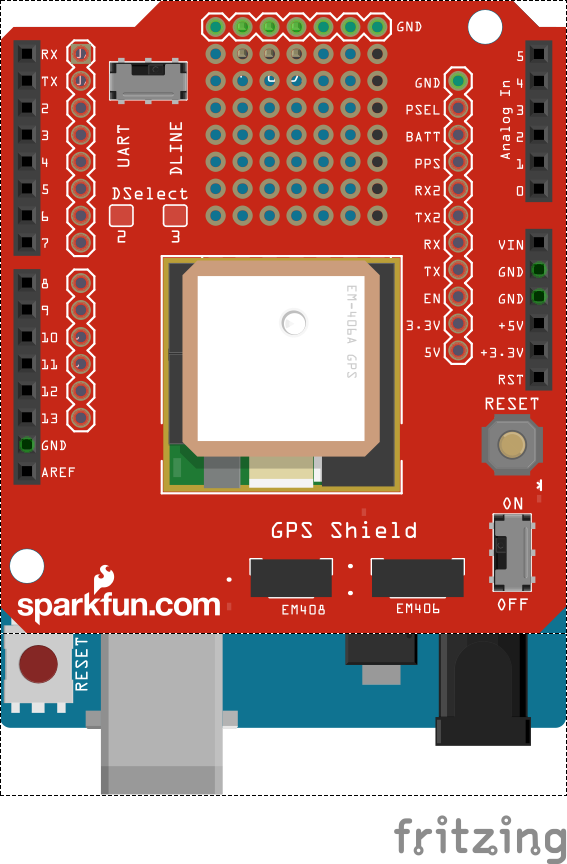
\includegraphics[width=0.3\textwidth]{figuras/arduinoGPS_bb.png}
    \caption{Shield GPS acoplado a um Arduino UNO R3}
    \label{fig:gps:vaa}
\end{figure}


/***DESCREVER***/

\begin{figure}[H]
    \centering
    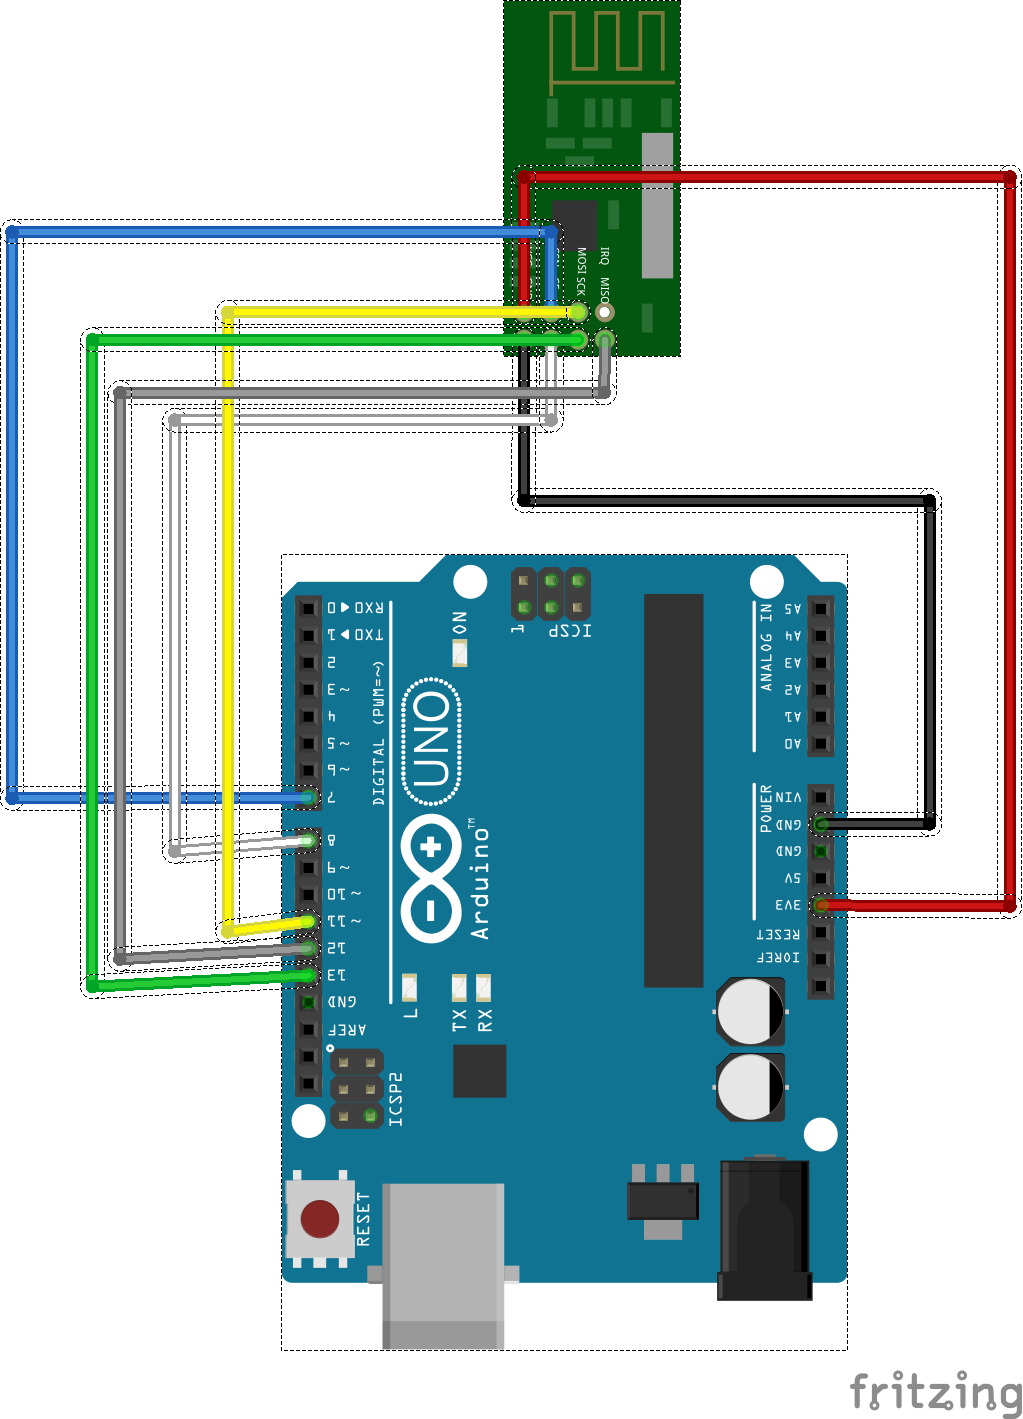
\includegraphics[width=0.5\textwidth]{figuras/radio_bb.png}
    \caption{Esquema do chassi}
    \label{fig:sketchup:vaa}
\end{figure}

\begin{figure}[H]
    \centering
    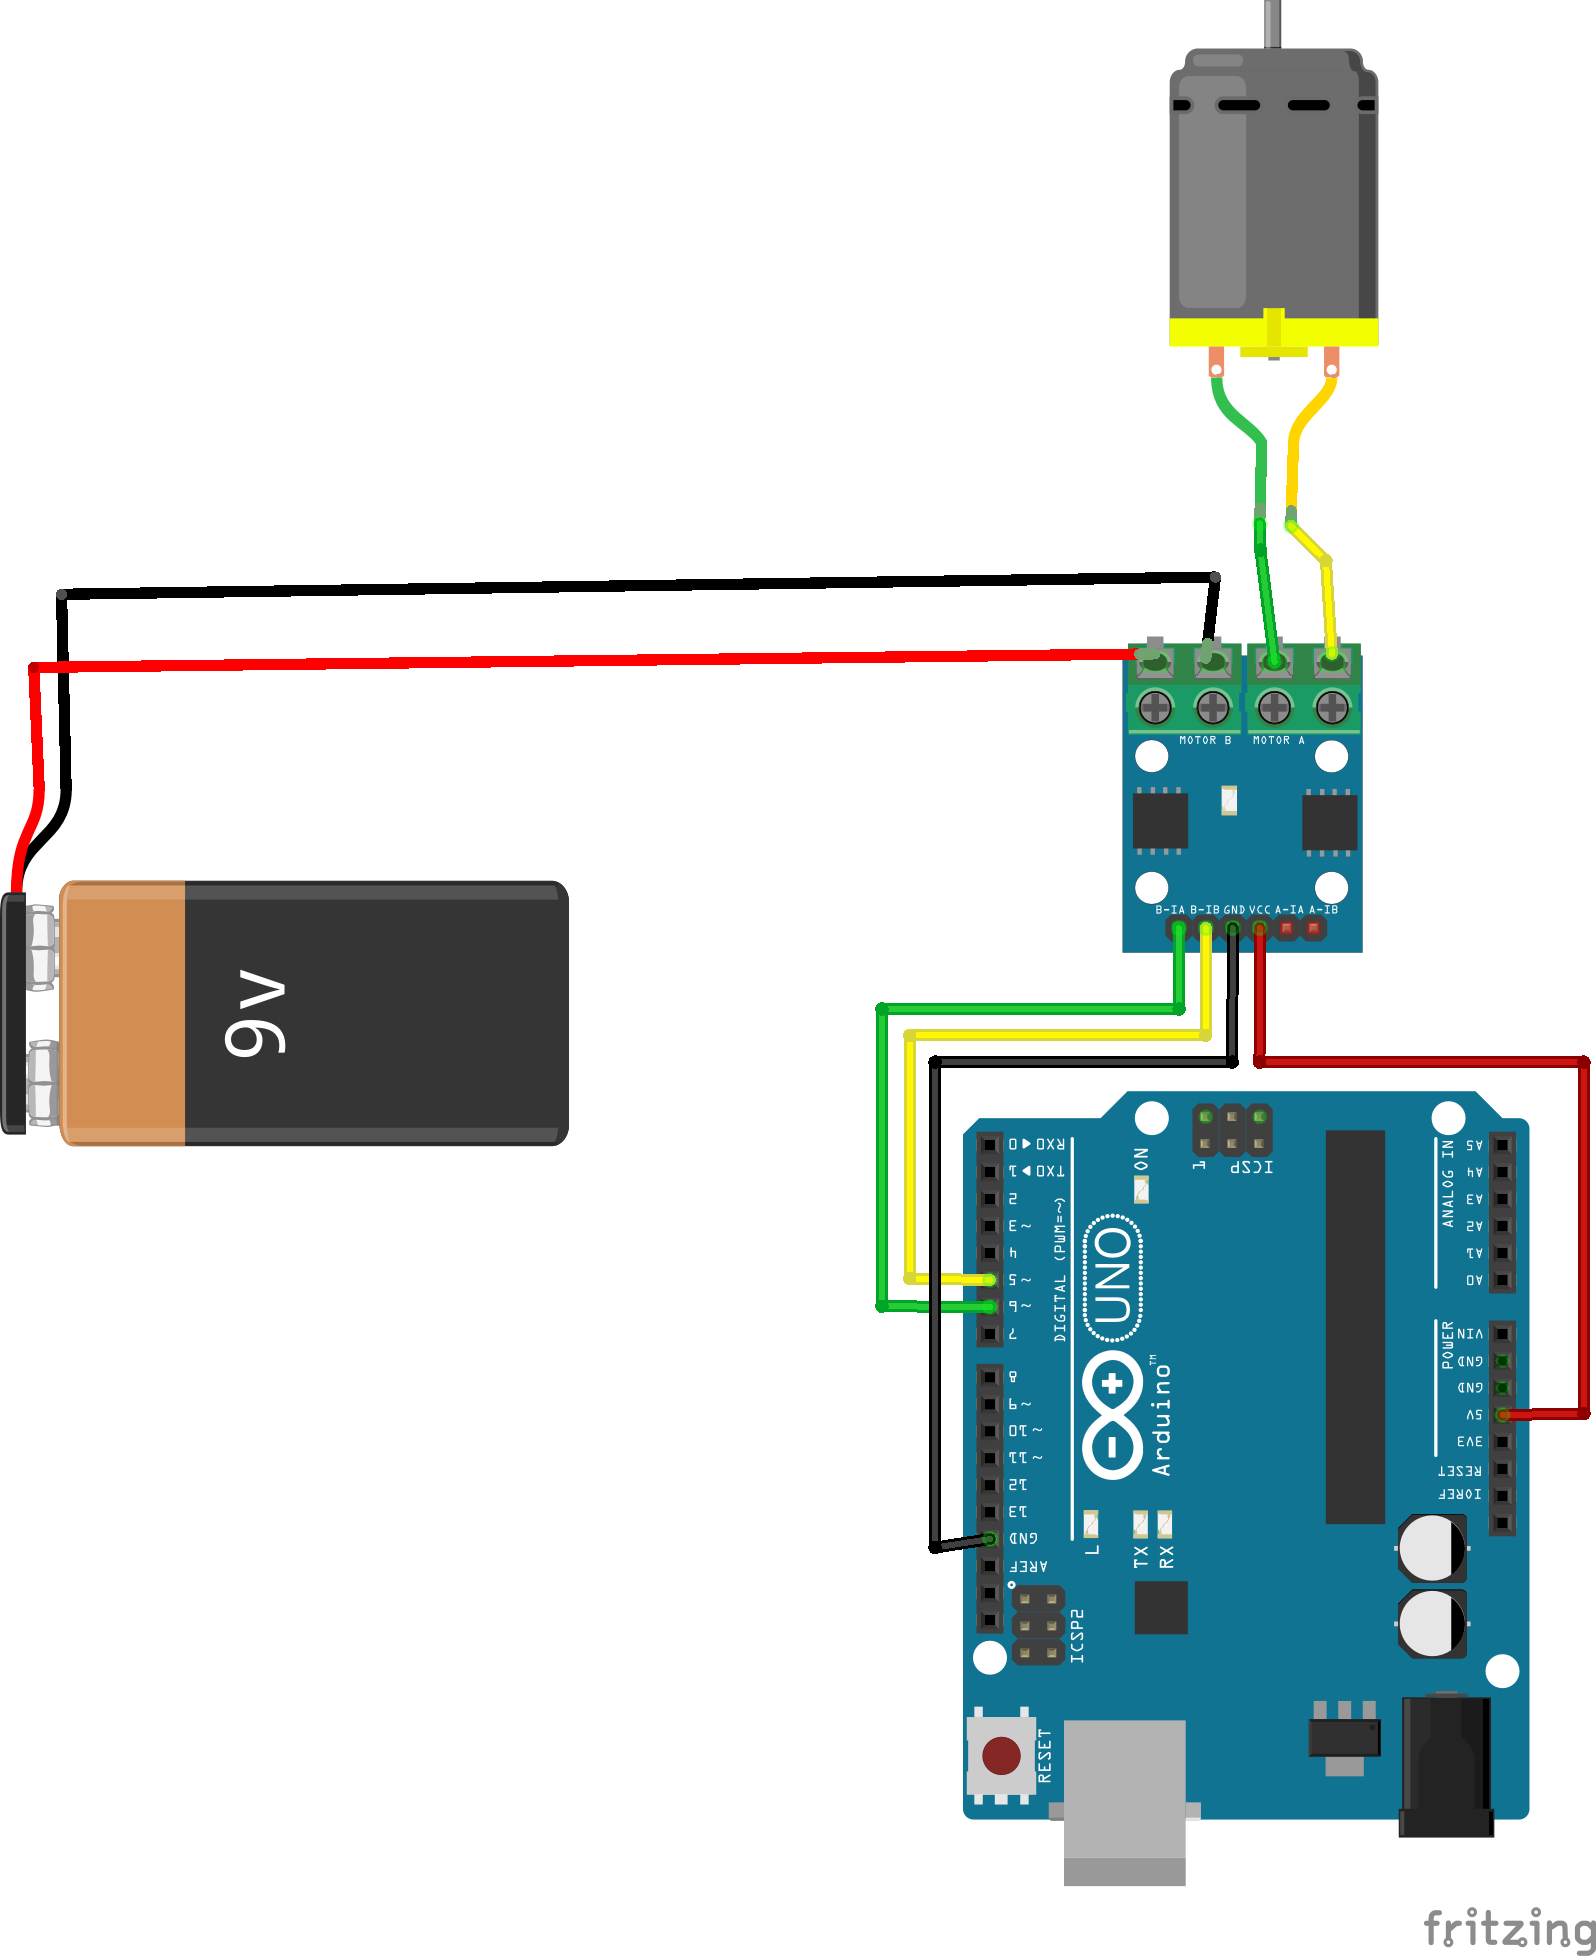
\includegraphics[width=0.5\textwidth]{figuras/motor_bb.png}
    \caption{Esquema do chassi}
    \label{fig:sketchup:vaa}
\end{figure}

A fim de operar esse veículo durante horas, será necessário criar um sistema fotovoltaico capaz de alimentar os componentes, bem como armazenar energia em baterias para que o mesmo continue operando mesmo em condições de baixa luminosidade ou até mesmo durante a noite. Para tal, devemos obter as especificações quanto ao consumo elétrico de cada componente, a fim de calcular qual o gasto, a autonomia do sistema, bem como os demais componentes a serem utilizados.

De inicio, deve-se quantificar, bem como obter os dados de todos os componentes do sistema, os quais estão presentes na tabela \ref{cap:proposta:tab:quantificar}:

%https://www.tablesgenerator.com/#

\begin{table}[]
\centering
\caption{Consumo por 8 horas de uso}
\label{cap:proposta:tab:quantificar}
\begin{tabular}{lll|l|l|}
\hline
\multicolumn{1}{|l|}{\textbf{Quantidade}} & \multicolumn{1}{l|}{\textbf{Descrição}}   & \textbf{Potência} & \textbf{Tempo de Uso} & \textbf{Consumo} \\ \hline
\multicolumn{1}{|l|}{6}                   & \multicolumn{1}{l|}{Arduino UNO R3}       & 0,54W             & 8 horas               & 4,32W            \\ \hline
\multicolumn{1}{|l|}{2}                   & \multicolumn{1}{l|}{Raspberry Pi}         & 1,2               & 8                     & 9,6W             \\ \hline
\multicolumn{1}{|l|}{1}                   & \multicolumn{1}{l|}{Motor elétrico 1/4hp} & 127w             & 8                     & 1016         \\ \hline
\multicolumn{1}{|l|}{1}                   & \multicolumn{1}{l|}{Motor elétrico}       & 30w               & 8                     & 240w             \\ \hline
\multicolumn{1}{|l|}{1}                   & \multicolumn{1}{l|}{NRF24L01}             & 0,115W            & 8                     & 0,92w            \\ \hline
\multicolumn{1}{|l|}{3}                   & \multicolumn{1}{l|}{HC-SR04}              & 0,015             & 8                     & 0,12w            \\ \hline
\multicolumn{1}{|l|}{1}                   & \multicolumn{1}{l|}{GPS shield}           & 0,02w             & 8                     & 0,16w            \\ \hline
                                          &                                           &                   & \textbf{Total}        & 1271,12w      \\ \cline{4-5} 
\end{tabular}
\end{table}

Na tabela acima obtemos o consumo total de todos os componentes durante um período de 8 horas. A escolha o Inversor de Corrente Autônomo deve obedecer a uma faixa de potência continua entre 226,98W e 317,78W, baseando-se no calculo feito a partir da potencia instantânea, vista na tabela \ref{cap:proposta:tab:instantaneo}: 

\begin{table}[]
\centering
\caption{Consumo instantâneo}
\label{cap:proposta:tab:instantaneo}
\begin{tabular}{l|l|l|}
\hline
\multicolumn{1}{|l|}{\textbf{Quantidade}} & \textbf{Descrição}   & \textbf{Potência} \\ \hline
\multicolumn{1}{|l|}{6}                   & Arduino UNO R3       & 0,54W             \\ \hline
\multicolumn{1}{|l|}{2}                   & Raspberry Pi         & 1,2               \\ \hline
\multicolumn{1}{|l|}{1}                   & Motor elétrico 1/4hp & 127w             \\ \hline
\multicolumn{1}{|l|}{1}                   & Motor elétrico       & 30w               \\ \hline
\multicolumn{1}{|l|}{1}                   & NRF24L01             & 0,115W            \\ \hline
\multicolumn{1}{|l|}{3}                   & HC-SR04              & 0,015             \\ \hline
\multicolumn{1}{|l|}{1}                   & GPS shield           & 0,02w             \\ \hline
                                          & \textbf{Total:}      & 158,89        \\ \cline{2-3} 
\end{tabular}
\end{table}
Onde, calculamos:
\[F_{max}=317,78w\] e \[F_{min}=226,98w\]
Referentes à faixa de operação com folga para o inversor autônomo. 

A seguir, calculamos o valor da energia gerada pelo sistema, dada uma eficiência máxima do inversor autônomo de 90\%, bem como a sua tensão de 24V:
\[ED =\frac{Consumo Diário}{Eficiência Máxima}\]
\[ED = \frac{1271,12}{0,9}\]
\[ED = 1412,35\]
Com isso, podemos calcular a energia real da instalação, sendo:
\[ER=\frac{ED}{R}\]
\[ER=\frac{1412,35}{0,89}\]
\[ER=1587\]

Para realizarmos os cálculos, assumimos os valores hipotéticos a uma bateria com as seguintes características apresentadas na tabela \ref{cap:proposta:tab:bateria}:
\begin{table}[h]
\centering
\caption{Bateria hipotética}
\label{cap:proposta:tab:bateria}
\begin{tabular}{|l|l|}
\hline
\multicolumn{2}{|c|}{\textbf{Bateria Hipotética}} \\ \hline
\textbf{Capacidade Real}          & 210Ah         \\ \hline
\textbf{Vb}                       & 12V           \\ \hline
\textbf{CN}                       & 105Ah         \\ \hline
\textbf{Pd}                       & 0,6           \\ \hline
\end{tabular}
\end{table}

Por fim, calcula-se o valor da capacidade útil do banco de baterias, assumindo que N terá o valor de $\frac{1}{24}$*8, adaptando a formula a consumo por horas. Temos que:
\[CU=\frac{ER*N}{Vi}\]
\[CU=\frac{1587*0,333}{24}\]
\[CU=22,03\]
Atentando-se de que as baterias não podem ser descarregadas em sua totalidade, calcula-se a carga real:
\[CR=\frac{CU}{PD}\]
\[CR=\frac{22,03}{0,6}\]
\[CR=36,71Ah\]
Finalmente, calcula-se o numero de baterias a serem utilizadas pelo sistema, tanto em série como em paralelo:
\[NB=\left ( \frac{CR}{CN} \right )*\left ( \frac{Vi}{VB} \right )\]
\[NB=\left ( \frac{36,71}{105} \right )*\left ( \frac{24}{12} \right )\]
\[NB=0,699\]
Como o resultado mostra, uma bateria será o suficiente para todo o sistema, e segundo os cálculos, com sobra.

 % Esse capítulo e nome é apenas uma sugestão (bom para TCC 1).
% ATENÇÃO - veja com o seu orientador se você vai ter este capítulo e se este vai ter nome!
\chapter{Metodologia}
\label{cap:metodologia}
Neste capítulo serão discutidos quais foram os passos já tomados e quais serão os passos para a elaboração deste trabalho, desde as pesquisas realizadas para o material bibliográfico, bem como um planejamento das futuras etapas, como pode ser observado na figura \ref{fig:metodologia:etapas} representando as etapas do trabalho. 

\begin{figure}[H]
    \centering
    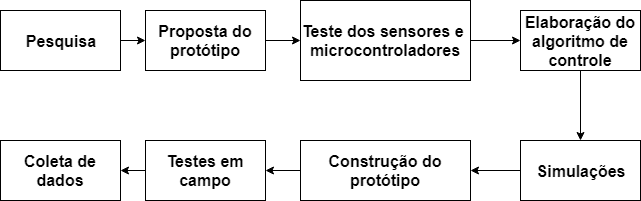
\includegraphics[width=0.8\textwidth]{figuras/metodologia.png}
    \caption{Fluxograma de etapas}
    \label{fig:metodologia:etapas}
\end{figure}

Com o tema definido, foram pesquisados artigos relacionados ao projeto de sistemas fotovoltaicos, o êxodo rural brasileiro, a mecanização do campo e agricultura de precisão, bem como trabalhos científicos com temáticas relacionadas a automação do  maquinário, da construção de protótipos, técnicas utilizadas em relação a movimentação dos veículos. A seguir, foram idealizados os componentes, bem como o chassi do veículo proposto. Durante a busca por trabalhos relacionados, foram usadas diversas bases de dados, tais como  \textit{Institute of Electrical and Electronics Engineers(IEEE) Xplore\footnote{https://ieeexplore.ieee.org/Xplore/home.jsp}, Google Scholar\footnote{https://scholar.google.com.br/}}, dentre outros bancos. 

A elaboração do protótipo foi feita em base das características de conceitos já testados em trabalhos % Esse capítulo e nome é apenas uma sugestão.
%\include{capitulos/cap-experimentos-resultados} % Esse capítulo e nome é apenas uma sugestão.
%\include{capitulos/cap-conclusoes} % Esse capítulo e nome é apenas uma sugestão.

% Apendices.
%\appendix
%\chapter{Instalação de Ferramentas}
\label{ape:instalacao:ferramentas}

Os apêndices são usados para disponibilizar materiais extras que por questões de espaço ou estilo de escrita não foram colocados diretamente no texto. Por exemplo, \textit{scripts}, instruções de instalação das ferramentas utilizadas pelo trabalho, partes de código fonte e questionários que tenham sido aplicados, tabelas com resultados...

(ATENÇÃO - veja com o seu orientador se é necessário disponibilizar algum material extra sobre algum capítulo em anexo!)



%bibliografia
\bibliographystyle{abntex2-alf}
\bibliography{main} % geração automática das referências a partir do arquivo main.bib

\backmatter
\end{document}
